\documentclass[../main]{subfiles}

\questiontrue
\solutiontrue
\begin{document}
    \ifquestion
    
    
    \section{Nill in the Telescope Wonderland}
	
Nill das Graças, as a child, was fascinated by telescopes! He lived in the countryside of Maranhão and had no one to teach him the techniques and tricks for handling the instruments, so he was forced to learn everything on his own. Follow Nill on his optical journey until he becomes the great astronomer he would eventually be.
	
\begin{doublespace}
		
		\begin{large}
			\textbf{Part A: Refracting Telescopes}
		\end{large}
		
\end{doublespace}
	
Nill began his path with refracting telescopes. The boy was very fond of geometric optics, so he soon thought of creating his first telescope based on his knowledge of how lenses work. Consider the setup designed by him:
	
	\begin{figure}[htpb]
	    \centering

\tikzset{every picture/.style={line width=0.75pt}} %set default line width to 0.75pt        

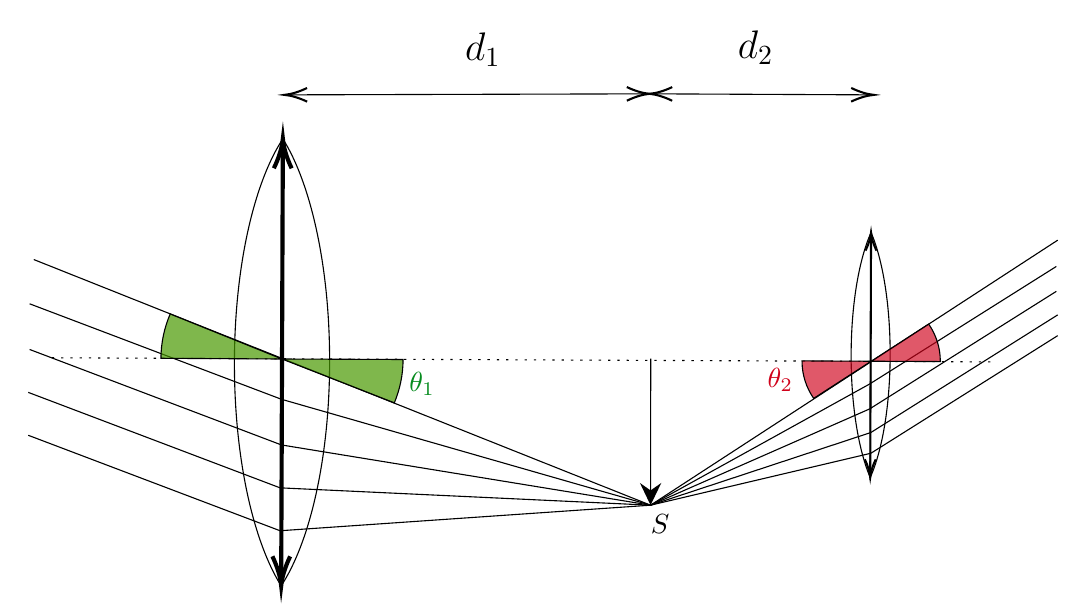
\begin{tikzpicture}[x=0.75pt,y=0.75pt,yscale=-1,xscale=1]
%uncomment if require: \path (0,408); %set diagram left start at 0, and has height of 408

%Shape: Chord [id:dp6567840789154635] 
\draw   (148.2,317.23) .. controls (134.72,295.71) and (125.67,255.82) .. (125.67,210.17) .. controls (125.67,163.61) and (135.08,123.04) .. (149.01,101.84) -- cycle ;
%Shape: Chord [id:dp6535665143076457] 
\draw   (149.01,101.84) .. controls (162.49,123.37) and (171.54,163.26) .. (171.54,208.9) .. controls (171.54,255.46) and (162.12,296.03) .. (148.2,317.23) -- cycle ;
%Shape: Chord [id:dp5311058754795721] 
\draw   (432,265.02) .. controls (426.43,252.03) and (422.8,230.64) .. (422.8,206.46) .. controls (422.8,181.7) and (426.61,159.87) .. (432.4,146.98) -- cycle ;
%Shape: Chord [id:dp8817014001653087] 
\draw   (432.4,146.98) .. controls (437.97,159.97) and (441.6,181.36) .. (441.6,205.55) .. controls (441.6,230.31) and (437.79,252.14) .. (432,265.02) -- cycle ;
%Straight Lines [id:da8230960559395764] 
\draw [line width=1.5]    (148.21,314.23) -- (149,104.84) ;
\draw [shift={(149.01,101.84)}, rotate = 90.22] [color={rgb, 255:red, 0; green, 0; blue, 0 }  ][line width=1.5]    (14.21,-4.28) .. controls (9.04,-1.82) and (4.3,-0.39) .. (0,0) .. controls (4.3,0.39) and (9.04,1.82) .. (14.21,4.28)   ;
\draw [shift={(148.2,317.23)}, rotate = 270.22] [color={rgb, 255:red, 0; green, 0; blue, 0 }  ][line width=1.5]    (14.21,-4.28) .. controls (9.04,-1.82) and (4.3,-0.39) .. (0,0) .. controls (4.3,0.39) and (9.04,1.82) .. (14.21,4.28)   ;
%Straight Lines [id:da28416750192252227] 
\draw [line width=0.75]    (432.01,263.02) -- (432.39,148.98) ;
\draw [shift={(432.4,146.98)}, rotate = 90.19] [color={rgb, 255:red, 0; green, 0; blue, 0 }  ][line width=0.75]    (8.74,-2.63) .. controls (5.56,-1.12) and (2.65,-0.24) .. (0,0) .. controls (2.65,0.24) and (5.56,1.12) .. (8.74,2.63)   ;
\draw [shift={(432,265.02)}, rotate = 270.19] [color={rgb, 255:red, 0; green, 0; blue, 0 }  ][line width=0.75]    (8.74,-2.63) .. controls (5.56,-1.12) and (2.65,-0.24) .. (0,0) .. controls (2.65,0.24) and (5.56,1.12) .. (8.74,2.63)   ;
%Straight Lines [id:da6155864639540956] 
\draw  [dash pattern={on 0.84pt off 2.51pt}]  (37.67,207.34) -- (492.33,209.34) ;
%Straight Lines [id:da5641496574728848] 
\draw    (326.25,207.7) -- (326.17,275.37) ;
\draw [shift={(326.17,278.37)}, rotate = 270.07] [fill={rgb, 255:red, 0; green, 0; blue, 0 }  ][line width=0.08]  [draw opacity=0] (10.72,-5.15) -- (0,0) -- (10.72,5.15) -- (7.12,0) -- cycle    ;
%Straight Lines [id:da5706739036006734] 
\draw    (29,160.01) -- (326.17,278.37) ;
%Straight Lines [id:da7486832943836399] 
\draw    (27,181.34) -- (148.33,227.34) ;
%Straight Lines [id:da028789208443993797] 
\draw    (27,203.34) -- (148.33,249.34) ;
%Straight Lines [id:da4166686391844716] 
\draw    (26.33,224.01) -- (147.67,270.01) ;
%Straight Lines [id:da2642747419253908] 
\draw    (26.33,244.68) -- (147.67,290.68) ;
%Straight Lines [id:da6917204761992566] 
\draw    (148.33,227.34) -- (326.17,278.37) ;
%Straight Lines [id:da5195927423081532] 
\draw    (148.33,249.34) -- (326.17,278.37) ;
%Straight Lines [id:da14657861425565777] 
\draw    (147.67,270.01) -- (326.17,278.37) ;
%Straight Lines [id:da08928459028770952] 
\draw    (147.67,290.68) -- (326.17,278.37) ;
%Straight Lines [id:da2085747203873265] 
\draw    (326.17,278.37) -- (522.33,150.68) ;
%Straight Lines [id:da09771274926589246] 
\draw    (431.67,220.01) -- (521.67,163.34) ;
%Straight Lines [id:da050864756884048345] 
\draw    (431.67,232.01) -- (521.67,175.34) ;
%Straight Lines [id:da25566998832836774] 
\draw    (432.33,253.34) -- (522.33,196.68) ;
%Straight Lines [id:da77778735894295] 
\draw    (432.33,243.34) -- (522.33,186.68) ;
%Straight Lines [id:da6180573934087692] 
\draw    (326.17,278.37) -- (431.67,220.01) ;
%Straight Lines [id:da7509861631177577] 
\draw    (326.17,278.37) -- (431.67,232.01) ;
%Straight Lines [id:da541361570449375] 
\draw    (326.17,278.37) -- (432.33,243.34) ;
%Straight Lines [id:da3370540738128609] 
\draw    (326.17,278.37) -- (432.33,253.34) ;
%Shape: Pie [id:dp23882155680095596] 
\draw  [fill={rgb, 255:red, 72; green, 152; blue, 0 }  ,fill opacity=0.7 ] (90.27,207.59) .. controls (90.32,200.02) and (91.9,192.81) .. (94.74,186.22) -- (148.6,207.94) -- cycle ;
%Shape: Pie [id:dp24354383277391523] 
\draw  [fill={rgb, 255:red, 72; green, 152; blue, 0 }  ,fill opacity=0.7 ] (206.93,208.17) .. controls (206.9,215.55) and (205.41,222.6) .. (202.72,229.06) -- (148.6,207.94) -- cycle ;
%Shape: Pie [id:dp22078911610616148] 
\draw  [fill={rgb, 255:red, 208; green, 2; blue, 27 }  ,fill opacity=0.66 ] (404.76,226.91) .. controls (401.22,221.79) and (399.15,215.63) .. (399.15,209.01) .. controls (399.15,208.95) and (399.15,208.9) .. (399.15,208.85) -- (432.46,209.01) -- cycle ;
%Shape: Pie [id:dp7824457237361571] 
\draw  [fill={rgb, 255:red, 208; green, 2; blue, 27 }  ,fill opacity=0.66 ] (460.16,191.1) .. controls (463.7,196.22) and (465.77,202.38) .. (465.77,209.01) .. controls (465.77,209.06) and (465.77,209.12) .. (465.77,209.17) -- (432.46,209.01) -- cycle ;
%Straight Lines [id:da23306702401744328] 
\draw    (151.75,80.67) -- (323.67,80.18) ;
\draw [shift={(325.67,80.17)}, rotate = 179.84] [color={rgb, 255:red, 0; green, 0; blue, 0 }  ][line width=0.75]    (10.93,-3.29) .. controls (6.95,-1.4) and (3.31,-0.3) .. (0,0) .. controls (3.31,0.3) and (6.95,1.4) .. (10.93,3.29)   ;
\draw [shift={(149.75,80.68)}, rotate = 359.84] [color={rgb, 255:red, 0; green, 0; blue, 0 }  ][line width=0.75]    (10.93,-3.29) .. controls (6.95,-1.4) and (3.31,-0.3) .. (0,0) .. controls (3.31,0.3) and (6.95,1.4) .. (10.93,3.29)   ;
%Straight Lines [id:da26069169894475896] 
\draw    (327.67,80.18) -- (431.75,80.67) ;
\draw [shift={(433.75,80.68)}, rotate = 180.27] [color={rgb, 255:red, 0; green, 0; blue, 0 }  ][line width=0.75]    (10.93,-3.29) .. controls (6.95,-1.4) and (3.31,-0.3) .. (0,0) .. controls (3.31,0.3) and (6.95,1.4) .. (10.93,3.29)   ;
\draw [shift={(325.67,80.17)}, rotate = 0.27] [color={rgb, 255:red, 0; green, 0; blue, 0 }  ][line width=0.75]    (10.93,-3.29) .. controls (6.95,-1.4) and (3.31,-0.3) .. (0,0) .. controls (3.31,0.3) and (6.95,1.4) .. (10.93,3.29)   ;

% Text Node
\draw (208.75,213.19) node [anchor=north west][inner sep=0.75pt]  [color={rgb, 255:red, 6; green, 139; blue, 30 }  ,opacity=1 ]  {$\theta _{1}$};
% Text Node
\draw (381.33,211.14) node [anchor=north west][inner sep=0.75pt]  [color={rgb, 255:red, 208; green, 2; blue, 27 }  ,opacity=1 ]  {$\theta _{2}$};
% Text Node
\draw (325,281.47) node [anchor=north west][inner sep=0.75pt]    {$S$};
% Text Node
\draw (235.5,49.57) node [anchor=north west][inner sep=0.75pt]  [font=\Large]  {$d_{1}$};
% Text Node
\draw (367,48.57) node [anchor=north west][inner sep=0.75pt]  [font=\Large]  {$d_{2}$};


\end{tikzpicture}
	    \caption{The interior of Nill's telescope and the functioning of the lenses in the deviation of light}
	    \label{fig:tele1}
	\end{figure}

	
	A recurring approximation is that the rays from the observed objects (stars, planets, among others) strike the objective lens—the larger one in the previous figure—in a parallel manner, since due to the great distances their angular size is close to zero. The telescope is also adjusted so that the rays exiting through the eyepiece—the smaller one in the image—also emerge parallel, in order to preserve the proportions of the original image.
	
	Nill knows and masters the lensmaker's equation:
	
	\begin{equation}
	\frac{1}{p}+\frac{1}{p'}=(n-1)\left(\frac{1}{R_1}+\frac{1}{R_2}\right)
	\end{equation}
	
	\ut{A.1} Knowing that Nill used glass to manufacture the lenses $(n=1.5)$, that the radius of curvature of the faces of the objective lens is $70$ cm and that of the faces of the eyepiece is $10$ cm, determine the focal lengths of each lens.
	
	
	\ut{A.2} Find the distances $d_1$ and $d_2$ and the length of the telescope.
	
	
	\ut{A.3} Find a relation between the angles $\theta_1$ and $\theta_2$. From this, argue how to find the angular magnification of the telescope for an object close to the lens axis. Show this value.
	
	
	\ut{A.4} Nill also measured the diameter of each lens: $D_{ob}=7.6$ cm and $D_{oc}=1$ cm. Knowing that each lens has an absorbance of $\epsilon=0.09$, what is the limiting magnitude of Nill's improvised telescope? The interior of the telescope is coated with black pigment that absorbs the incident radiation.
	\begin{itemize}
		\item Limiting magnitude of observation of the human eye = 6.
		\item Diameter of the human pupil = 6 mm.
		\item Consider that the radiation comes parallel to the lens axis (represented by the horizontal line).
		\item Hint: make the smallest possible number of assumptions!
	\end{itemize}
	
	Note that in this arrangement the final image is inverted along the vertical axis. To obtain an image with the correct orientation, a diverging eyepiece would be necessary.
	
	\begin{doublespace}
		
		
		\begin{large}
			\textbf{Part B: Reflecting Telescopes}
		\end{large}
		
	\end{doublespace}
	
	
	Continuing his studies, Nill moved on to a new type of telescope: reflectors. In these, instead of lenses, mirrors shaped into specific forms are used to correctly direct and focus the light to the observer's eyes.
	
	To this end, Nill decided to learn more about the reflective properties of conic sections.
	
	
	\ut{B.1} Consider an ellipsoid mirrored on the inside. Prove that any ray of light that originates from one of the foci of the conic reflects and strikes its other focus. Hint: solving the problem backwards, that is, proving that the path that connects one focus to the other and touches the conic once can be realized by a ray of light, may be much more practical.
	
	
	\ut{B.2} Consider a paraboloid mirrored on the inside (concave part). Prove that any ray of light that originates from the focus of the parabola reflects and emerges parallel to its axis. Hint: since you already know the result for ellipses from the previous item, could that help you here?
	
	
	\ut{B.3} Consider a hyperboloid—half of a hyperboloid, that is, consisting of only one of the two branches of the curve—mirrored on the outside (convex part). Prove that any ray of light that is directed toward the focus of this half reflects off the curve and strikes the focus of the other half (which was not considered).
	
	
	Nill built his first telescope with a Cassegrain focus, which uses a parabolic primary mirror and a hyperbolic secondary mirror, as shown in Figure \ref{fig:cassegrain}.


	\begin{figure}[htpb]
	    \centering
	    
\tikzset{every picture/.style={line width=0.75pt}} %set default line width to 0.75pt        

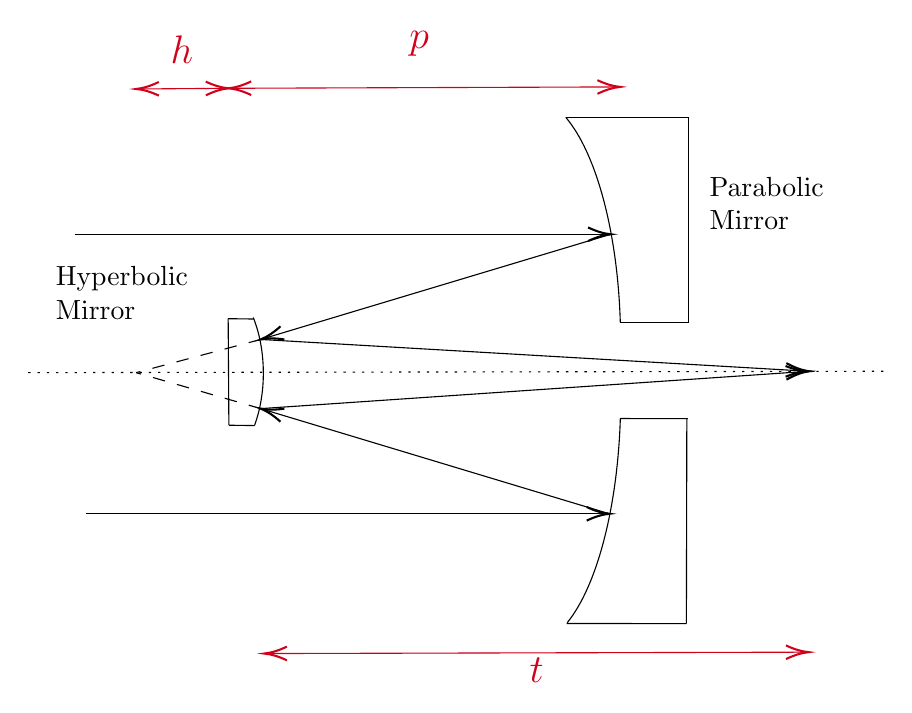
\begin{tikzpicture}[x=0.75pt,y=0.75pt,yscale=-1,xscale=1]
%uncomment if require: \path (0,408); %set diagram left start at 0, and has height of 408

%Straight Lines [id:da7103196653386519] 
\draw    (368,83) -- (427,83) ;
%Straight Lines [id:da456483423352092] 
\draw    (427,83) -- (427,181.76) ;
%Straight Lines [id:da41716859256351757] 
\draw    (394.26,181.76) -- (427.5,181.76) ;
%Shape: Arc [id:dp4646169466417964] 
\draw  [draw opacity=0] (368,83) .. controls (382.48,100.1) and (392.89,137.48) .. (394.26,181.76) -- (350.24,191.67) -- cycle ; \draw   (368,83) .. controls (382.48,100.1) and (392.89,137.48) .. (394.26,181.76) ;  
%Straight Lines [id:da9481690217207581] 
\draw    (368.37,326.85) -- (426.1,326.93) ;
%Straight Lines [id:da7760351753663124] 
\draw    (426.1,326.93) -- (426.31,228.16) ;
%Straight Lines [id:da37660161614238885] 
\draw    (394.27,228.12) -- (426.8,228.16) ;
%Shape: Arc [id:dp6016749426594743] 
\draw  [draw opacity=0] (368.7,326.46) .. controls (382.76,309.17) and (392.89,271.94) .. (394.28,227.91) -- (351.23,218.15) -- cycle ; \draw   (368.7,326.46) .. controls (382.76,309.17) and (392.89,271.94) .. (394.28,227.91) ;  
%Straight Lines [id:da23128777489749663] 
\draw  [dash pattern={on 0.84pt off 2.51pt}]  (109,206.01) -- (521,205.34) ;
%Straight Lines [id:da3532070262121205] 
\draw    (205.33,180.01) -- (205.67,231.34) ;
%Straight Lines [id:da8141414988368341] 
\draw    (205.33,180.01) -- (217.67,180.17) ;
%Straight Lines [id:da5697287616147251] 
\draw    (205.67,231.34) -- (218,231.51) ;
%Shape: Arc [id:dp07912069910025843] 
\draw  [draw opacity=0] (217.43,179.42) .. controls (220.44,187.02) and (222.21,196.06) .. (222.27,205.77) .. controls (222.33,215.19) and (220.76,224.01) .. (218,231.51) -- (192.27,205.95) -- cycle ; \draw   (217.43,179.42) .. controls (220.44,187.02) and (222.21,196.06) .. (222.27,205.77) .. controls (222.33,215.19) and (220.76,224.01) .. (218,231.51) ;  
%Straight Lines [id:da18681206167208808] 
\draw    (131.33,139.34) -- (387.67,139.34) ;
\draw [shift={(389.67,139.34)}, rotate = 180] [color={rgb, 255:red, 0; green, 0; blue, 0 }  ][line width=0.75]    (10.93,-3.29) .. controls (6.95,-1.4) and (3.31,-0.3) .. (0,0) .. controls (3.31,0.3) and (6.95,1.4) .. (10.93,3.29)   ;
%Straight Lines [id:da3703873332157699] 
\draw    (389.67,139.34) -- (222.92,189.44) ;
\draw [shift={(221,190.01)}, rotate = 343.28] [color={rgb, 255:red, 0; green, 0; blue, 0 }  ][line width=0.75]    (10.93,-3.29) .. controls (6.95,-1.4) and (3.31,-0.3) .. (0,0) .. controls (3.31,0.3) and (6.95,1.4) .. (10.93,3.29)   ;
%Straight Lines [id:da7249710864949106] 
\draw    (137,274.01) -- (387,274.01) ;
\draw [shift={(389,274.01)}, rotate = 180] [color={rgb, 255:red, 0; green, 0; blue, 0 }  ][line width=0.75]    (10.93,-3.29) .. controls (6.95,-1.4) and (3.31,-0.3) .. (0,0) .. controls (3.31,0.3) and (6.95,1.4) .. (10.93,3.29)   ;
%Straight Lines [id:da8877428370960709] 
\draw    (389,274.01) -- (222.91,223.92) ;
\draw [shift={(221,223.34)}, rotate = 16.78] [color={rgb, 255:red, 0; green, 0; blue, 0 }  ][line width=0.75]    (10.93,-3.29) .. controls (6.95,-1.4) and (3.31,-0.3) .. (0,0) .. controls (3.31,0.3) and (6.95,1.4) .. (10.93,3.29)   ;
%Straight Lines [id:da6909106330926893] 
\draw    (221,190.01) -- (483,205.23) ;
\draw [shift={(485,205.34)}, rotate = 183.32] [color={rgb, 255:red, 0; green, 0; blue, 0 }  ][line width=0.75]    (10.93,-3.29) .. controls (6.95,-1.4) and (3.31,-0.3) .. (0,0) .. controls (3.31,0.3) and (6.95,1.4) .. (10.93,3.29)   ;
%Straight Lines [id:da1734537051971483] 
\draw    (221,223.34) -- (483,205.48) ;
\draw [shift={(485,205.34)}, rotate = 176.1] [color={rgb, 255:red, 0; green, 0; blue, 0 }  ][line width=0.75]    (10.93,-3.29) .. controls (6.95,-1.4) and (3.31,-0.3) .. (0,0) .. controls (3.31,0.3) and (6.95,1.4) .. (10.93,3.29)   ;
%Straight Lines [id:da4366821007736077] 
\draw  [dash pattern={on 4.5pt off 4.5pt}]  (221,190.01) -- (161,206.01) ;
%Straight Lines [id:da07200196058992936] 
\draw  [dash pattern={on 4.5pt off 4.5pt}]  (221,223.34) -- (161,206.01) ;
%Straight Lines [id:da5189243475923575] 
\draw [color={rgb, 255:red, 208; green, 2; blue, 27 }  ,draw opacity=1 ]   (163,69.33) -- (203.5,69.03) ;
\draw [shift={(205.5,69.01)}, rotate = 179.57] [color={rgb, 255:red, 208; green, 2; blue, 27 }  ,draw opacity=1 ][line width=0.75]    (10.93,-3.29) .. controls (6.95,-1.4) and (3.31,-0.3) .. (0,0) .. controls (3.31,0.3) and (6.95,1.4) .. (10.93,3.29)   ;
\draw [shift={(161,69.34)}, rotate = 359.57] [color={rgb, 255:red, 208; green, 2; blue, 27 }  ,draw opacity=1 ][line width=0.75]    (10.93,-3.29) .. controls (6.95,-1.4) and (3.31,-0.3) .. (0,0) .. controls (3.31,0.3) and (6.95,1.4) .. (10.93,3.29)   ;
%Straight Lines [id:da40713772795028613] 
\draw [color={rgb, 255:red, 208; green, 2; blue, 27 }  ,draw opacity=1 ]   (207.5,69) -- (392.17,68.35) ;
\draw [shift={(394.17,68.34)}, rotate = 179.8] [color={rgb, 255:red, 208; green, 2; blue, 27 }  ,draw opacity=1 ][line width=0.75]    (10.93,-3.29) .. controls (6.95,-1.4) and (3.31,-0.3) .. (0,0) .. controls (3.31,0.3) and (6.95,1.4) .. (10.93,3.29)   ;
\draw [shift={(205.5,69.01)}, rotate = 359.8] [color={rgb, 255:red, 208; green, 2; blue, 27 }  ,draw opacity=1 ][line width=0.75]    (10.93,-3.29) .. controls (6.95,-1.4) and (3.31,-0.3) .. (0,0) .. controls (3.31,0.3) and (6.95,1.4) .. (10.93,3.29)   ;
%Straight Lines [id:da4795303143392031] 
\draw [color={rgb, 255:red, 208; green, 2; blue, 27 }  ,draw opacity=1 ][fill={rgb, 255:red, 208; green, 2; blue, 27 }  ,fill opacity=1 ]   (224.67,341.34) -- (483,340.68) ;
\draw [shift={(485,340.68)}, rotate = 179.85] [color={rgb, 255:red, 208; green, 2; blue, 27 }  ,draw opacity=1 ][line width=0.75]    (10.93,-3.29) .. controls (6.95,-1.4) and (3.31,-0.3) .. (0,0) .. controls (3.31,0.3) and (6.95,1.4) .. (10.93,3.29)   ;
\draw [shift={(222.67,341.34)}, rotate = 359.85] [color={rgb, 255:red, 208; green, 2; blue, 27 }  ,draw opacity=1 ][line width=0.75]    (10.93,-3.29) .. controls (6.95,-1.4) and (3.31,-0.3) .. (0,0) .. controls (3.31,0.3) and (6.95,1.4) .. (10.93,3.29)   ;

% Text Node
\draw (176.33,42.4) node [anchor=north west][inner sep=0.75pt]  [font=\Large,color={rgb, 255:red, 208; green, 2; blue, 27 }  ,opacity=1 ]  {$h$};
% Text Node
\draw (291.33,40.07) node [anchor=north west][inner sep=0.75pt]  [font=\Large,color={rgb, 255:red, 208; green, 2; blue, 27 }  ,opacity=1 ]  {$p$};
% Text Node
\draw (349.33,342.41) node [anchor=north west][inner sep=0.75pt]  [font=\Large,color={rgb, 255:red, 208; green, 2; blue, 27 }  ,opacity=1 ]  {$t$};
% Text Node
\draw (121,153.67) node [anchor=north west][inner sep=0.75pt]   [align=left] {Hyperbolic\\Mirror};
% Text Node
\draw (436,110.67) node [anchor=north west][inner sep=0.75pt]   [align=left] {Parabolic\\Mirror};


\end{tikzpicture}
	    \caption{Image focusing apparatus with a Cassegrain focus, based on a parabolic mirror with a hole and a secondary hyperbolic mirror}
	    \label{fig:cassegrain}
	\end{figure}

	
	The young man knows all the parameters of the telescope and wishes to find other important relations for the operation of the instrument, as tabulated in Table \ref{tab:paramteles}.
	
	\begin{table}[htpb]
	    \centering
	    \caption{Telescope construction parameters}
        \begin{tabular}{c c} 
			\toprule
			Quantity & Value $(\unit{\milli \meter})$ \\
			\midrule
			$h$ & $233$ mm\\
		
			$p$ & $467$ mm\\

			$t$ & $534$ mm\\

			$D$ & $195$ mm \\
			\bottomrule
		\end{tabular}
	    
	    \label{tab:paramteles}
	\end{table}

	
	\ut{B.4} Starting from these data, find the focus of the primary mirror.
	
	
	\ut{B.5} Find a relation between the effective focus of the system and the focus of the primary mirror. Define effective focus as the focus of a converging lens that would generate the same final effect as the system, that is, the same final angular deviation of the rays.
	
	\ut{B.6} Find the focal ratio of the telescope.
	
	\ut{B.7} Each mirror has an absorbance of $\epsilon=0.05$, and the dimensions of the mirrors are adjusted so that parallel rays with the greatest possible separation that enter the tube are reflected at the edges of the mirrors. The hole in the primary mirror is adjusted to be aligned and smaller than the secondary mirror and large enough to allow all the radiation to pass through without obstruction so as to be focused into the observer's eye. In this way, find the limiting magnitude of the telescope. 
	
	After that, Nill continued his studies with image acquisition and processing devices, seeking to develop his own CCD! But that is already a story for another question.
	\clearpage
    
    \fi
    
    \ifsolution
    
    \section{Nill in the Telescope Wonderland}
	
	\begin{doublespace}
		
		
		\begin{large}
			\textbf{Part A: Refracting Telescopes}
		\end{large}
		
	\end{doublespace}
	
	\ut{A.1} As shown by the famous lens equation:
	
	$$\frac{1}{p}+\frac{1}{p'}=\frac{1}{f}$$
	
	We then know that, since in both cases $R_1=R_2=R$:
	
	$$f=\frac{R}{2(n-1)}$$
	
	As $n=1.5$, we find that $f=R$! Therefore: $f_{ob}=70 cm$ and $f_{oc}=10 cm$.
	
	
	\ut{A.2} In order for the conversion of parallel rays into the intermediate image and vice versa to occur, it is necessary that each distance be equal to the focal length of its respective lens; thus $d_1=70 cm$ and $d_2=10 cm$.
	
	
	\ut{A.3} From the image of the intermediate image, we can conclude that the length $l$ of the intermediate image can be obtained in two equivalent ways:
	
	$$\begin{cases}
		l=d_1 \tan{(\theta_1)} \\
		l=d_2 \tan{(\theta_2)} \\
	\end{cases}$$
	
	Thus we have $f_{ob} \tan{(\theta_1)}=f_{oc} \tan{(\theta_2)}$.
	
	Note that when the angle of the light rays is changed, the angular size of the object also changes. In this case, consider the scheme below, which presents the analysis of an object located on the lens axis and having an angular diameter of $2\theta_1$. One wishes to know the variation of this parameter after passing through the tube and reaching the observer's eye, as shown in Figure \ref{fig:tele1}.


	\begin{figure}[htpb]
	    \centering
	    

\tikzset{every picture/.style={line width=0.75pt}} %set default line width to 0.75pt        

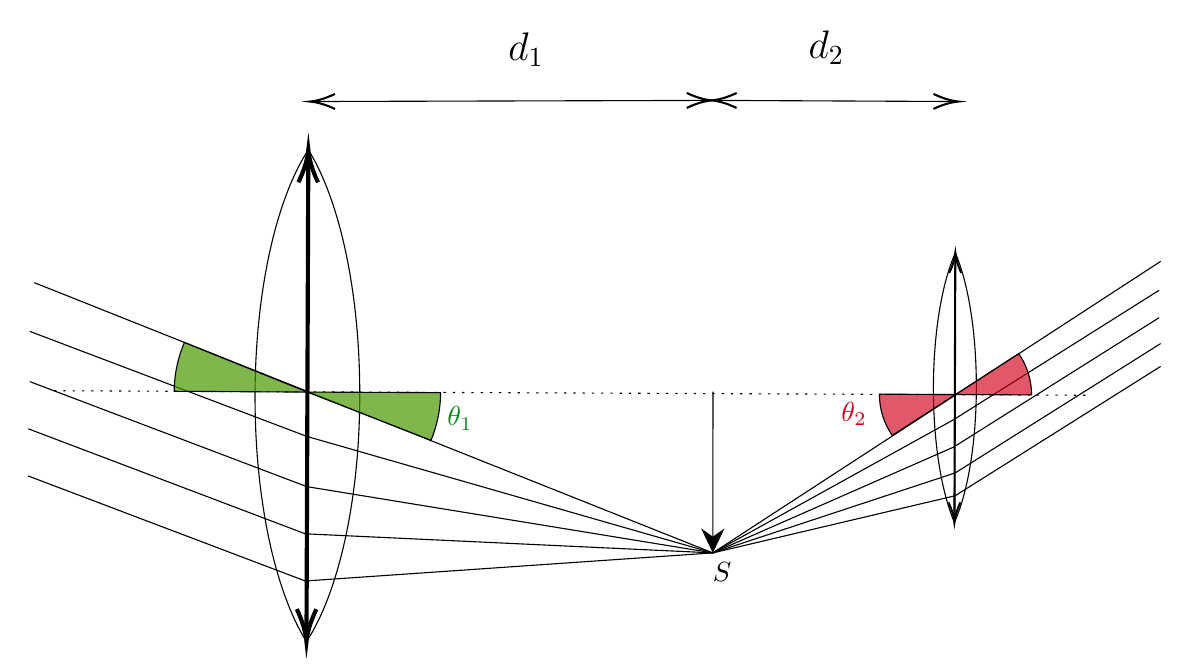
\begin{tikzpicture}[x=0.75pt,y=0.75pt,yscale=-1.1,xscale=1.1]
%uncomment if require: \path (0,408); %set diagram left start at 0, and has height of 408

%Shape: Chord [id:dp6567840789154635] 
\draw   (148.2,317.23) .. controls (134.72,295.71) and (125.67,255.82) .. (125.67,210.17) .. controls (125.67,163.61) and (135.08,123.04) .. (149.01,101.84) -- cycle ;
%Shape: Chord [id:dp6535665143076457] 
\draw   (149.01,101.84) .. controls (162.49,123.37) and (171.54,163.26) .. (171.54,208.9) .. controls (171.54,255.46) and (162.12,296.03) .. (148.2,317.23) -- cycle ;
%Shape: Chord [id:dp5311058754795721] 
\draw   (432,265.02) .. controls (426.43,252.03) and (422.8,230.64) .. (422.8,206.46) .. controls (422.8,181.7) and (426.61,159.87) .. (432.4,146.98) -- cycle ;
%Shape: Chord [id:dp8817014001653087] 
\draw   (432.4,146.98) .. controls (437.97,159.97) and (441.6,181.36) .. (441.6,205.55) .. controls (441.6,230.31) and (437.79,252.14) .. (432,265.02) -- cycle ;
%Straight Lines [id:da8230960559395764] 
\draw [line width=1.5]    (148.21,314.23) -- (149,104.84) ;
\draw [shift={(149.01,101.84)}, rotate = 90.22] [color={rgb, 255:red, 0; green, 0; blue, 0 }  ][line width=1.5]    (14.21,-4.28) .. controls (9.04,-1.82) and (4.3,-0.39) .. (0,0) .. controls (4.3,0.39) and (9.04,1.82) .. (14.21,4.28)   ;
\draw [shift={(148.2,317.23)}, rotate = 270.22] [color={rgb, 255:red, 0; green, 0; blue, 0 }  ][line width=1.5]    (14.21,-4.28) .. controls (9.04,-1.82) and (4.3,-0.39) .. (0,0) .. controls (4.3,0.39) and (9.04,1.82) .. (14.21,4.28)   ;
%Straight Lines [id:da28416750192252227] 
\draw [line width=0.75]    (432.01,263.02) -- (432.39,148.98) ;
\draw [shift={(432.4,146.98)}, rotate = 90.19] [color={rgb, 255:red, 0; green, 0; blue, 0 }  ][line width=0.75]    (8.74,-2.63) .. controls (5.56,-1.12) and (2.65,-0.24) .. (0,0) .. controls (2.65,0.24) and (5.56,1.12) .. (8.74,2.63)   ;
\draw [shift={(432,265.02)}, rotate = 270.19] [color={rgb, 255:red, 0; green, 0; blue, 0 }  ][line width=0.75]    (8.74,-2.63) .. controls (5.56,-1.12) and (2.65,-0.24) .. (0,0) .. controls (2.65,0.24) and (5.56,1.12) .. (8.74,2.63)   ;
%Straight Lines [id:da6155864639540956] 
\draw  [dash pattern={on 0.84pt off 2.51pt}]  (37.67,207.34) -- (492.33,209.34) ;
%Straight Lines [id:da5641496574728848] 
\draw    (326.25,207.7) -- (326.17,275.37) ;
\draw [shift={(326.17,278.37)}, rotate = 270.07] [fill={rgb, 255:red, 0; green, 0; blue, 0 }  ][line width=0.08]  [draw opacity=0] (10.72,-5.15) -- (0,0) -- (10.72,5.15) -- (7.12,0) -- cycle    ;
%Straight Lines [id:da5706739036006734] 
\draw    (29,160.01) -- (326.17,278.37) ;
%Straight Lines [id:da7486832943836399] 
\draw    (27,181.34) -- (148.33,227.34) ;
%Straight Lines [id:da028789208443993797] 
\draw    (27,203.34) -- (148.33,249.34) ;
%Straight Lines [id:da4166686391844716] 
\draw    (26.33,224.01) -- (147.67,270.01) ;
%Straight Lines [id:da2642747419253908] 
\draw    (26.33,244.68) -- (147.67,290.68) ;
%Straight Lines [id:da6917204761992566] 
\draw    (148.33,227.34) -- (326.17,278.37) ;
%Straight Lines [id:da5195927423081532] 
\draw    (148.33,249.34) -- (326.17,278.37) ;
%Straight Lines [id:da14657861425565777] 
\draw    (147.67,270.01) -- (326.17,278.37) ;
%Straight Lines [id:da08928459028770952] 
\draw    (147.67,290.68) -- (326.17,278.37) ;
%Straight Lines [id:da2085747203873265] 
\draw    (326.17,278.37) -- (522.33,150.68) ;
%Straight Lines [id:da09771274926589246] 
\draw    (431.67,220.01) -- (521.67,163.34) ;
%Straight Lines [id:da050864756884048345] 
\draw    (431.67,232.01) -- (521.67,175.34) ;
%Straight Lines [id:da25566998832836774] 
\draw    (432.33,253.34) -- (522.33,196.68) ;
%Straight Lines [id:da77778735894295] 
\draw    (432.33,243.34) -- (522.33,186.68) ;
%Straight Lines [id:da6180573934087692] 
\draw    (326.17,278.37) -- (431.67,220.01) ;
%Straight Lines [id:da7509861631177577] 
\draw    (326.17,278.37) -- (431.67,232.01) ;
%Straight Lines [id:da541361570449375] 
\draw    (326.17,278.37) -- (432.33,243.34) ;
%Straight Lines [id:da3370540738128609] 
\draw    (326.17,278.37) -- (432.33,253.34) ;
%Shape: Pie [id:dp23882155680095596] 
\draw  [fill={rgb, 255:red, 72; green, 152; blue, 0 }  ,fill opacity=0.7 ] (90.27,207.59) .. controls (90.32,200.02) and (91.9,192.81) .. (94.74,186.22) -- (148.6,207.94) -- cycle ;
%Shape: Pie [id:dp24354383277391523] 
\draw  [fill={rgb, 255:red, 72; green, 152; blue, 0 }  ,fill opacity=0.7 ] (206.93,208.17) .. controls (206.9,215.55) and (205.41,222.6) .. (202.72,229.06) -- (148.6,207.94) -- cycle ;
%Shape: Pie [id:dp22078911610616148] 
\draw  [fill={rgb, 255:red, 208; green, 2; blue, 27 }  ,fill opacity=0.66 ] (404.76,226.91) .. controls (401.22,221.79) and (399.15,215.63) .. (399.15,209.01) .. controls (399.15,208.95) and (399.15,208.9) .. (399.15,208.85) -- (432.46,209.01) -- cycle ;
%Shape: Pie [id:dp7824457237361571] 
\draw  [fill={rgb, 255:red, 208; green, 2; blue, 27 }  ,fill opacity=0.66 ] (460.16,191.1) .. controls (463.7,196.22) and (465.77,202.38) .. (465.77,209.01) .. controls (465.77,209.06) and (465.77,209.12) .. (465.77,209.17) -- (432.46,209.01) -- cycle ;
%Straight Lines [id:da23306702401744328] 
\draw    (151.75,80.67) -- (323.67,80.18) ;
\draw [shift={(325.67,80.17)}, rotate = 179.84] [color={rgb, 255:red, 0; green, 0; blue, 0 }  ][line width=0.75]    (10.93,-3.29) .. controls (6.95,-1.4) and (3.31,-0.3) .. (0,0) .. controls (3.31,0.3) and (6.95,1.4) .. (10.93,3.29)   ;
\draw [shift={(149.75,80.68)}, rotate = 359.84] [color={rgb, 255:red, 0; green, 0; blue, 0 }  ][line width=0.75]    (10.93,-3.29) .. controls (6.95,-1.4) and (3.31,-0.3) .. (0,0) .. controls (3.31,0.3) and (6.95,1.4) .. (10.93,3.29)   ;
%Straight Lines [id:da26069169894475896] 
\draw    (327.67,80.18) -- (431.75,80.67) ;
\draw [shift={(433.75,80.68)}, rotate = 180.27] [color={rgb, 255:red, 0; green, 0; blue, 0 }  ][line width=0.75]    (10.93,-3.29) .. controls (6.95,-1.4) and (3.31,-0.3) .. (0,0) .. controls (3.31,0.3) and (6.95,1.4) .. (10.93,3.29)   ;
\draw [shift={(325.67,80.17)}, rotate = 0.27] [color={rgb, 255:red, 0; green, 0; blue, 0 }  ][line width=0.75]    (10.93,-3.29) .. controls (6.95,-1.4) and (3.31,-0.3) .. (0,0) .. controls (3.31,0.3) and (6.95,1.4) .. (10.93,3.29)   ;

% Text Node
\draw (208.75,213.19) node [anchor=north west][inner sep=0.75pt]  [color={rgb, 255:red, 6; green, 139; blue, 30 }  ,opacity=1 ]  {$\theta _{1}$};
% Text Node
\draw (381.33,211.14) node [anchor=north west][inner sep=0.75pt]  [color={rgb, 255:red, 208; green, 2; blue, 27 }  ,opacity=1 ]  {$\theta _{2}$};
% Text Node
\draw (325,281.47) node [anchor=north west][inner sep=0.75pt]    {$S$};
% Text Node
\draw (235.5,49.57) node [anchor=north west][inner sep=0.75pt]  [font=\Large]  {$d_{1}$};
% Text Node
\draw (367,48.57) node [anchor=north west][inner sep=0.75pt]  [font=\Large]  {$d_{2}$};


\end{tikzpicture}
	\end{figure}
	
	In this way, it is observed that the size of the image is proportional to the angle $\theta$, so we find that the magnification factor is $A=\dfrac{\theta_2}{\theta_1}$:
	
	$$A=\frac{2\arctan{\left(\frac{f_{ob}}{f_{oc}}\tan{\left(\frac{\delta}{2}\right)}\right)}}{\delta}$$
	
	With $\delta=2\theta_1$ being the initial angular diameter. In common cases, such angles are infinitesimal, so we can approximate $\tan{(\theta)} \approx \theta$, thus we find the famous relation:
	
	$$A=\frac{f_{ob}}{f_{oc}}$$
	
	\ut{A.4} Check the following scheme:

    \begin{figure}[htpb]
        \centering
        

\tikzset{every picture/.style={line width=0.75pt}} %set default line width to 0.75pt        

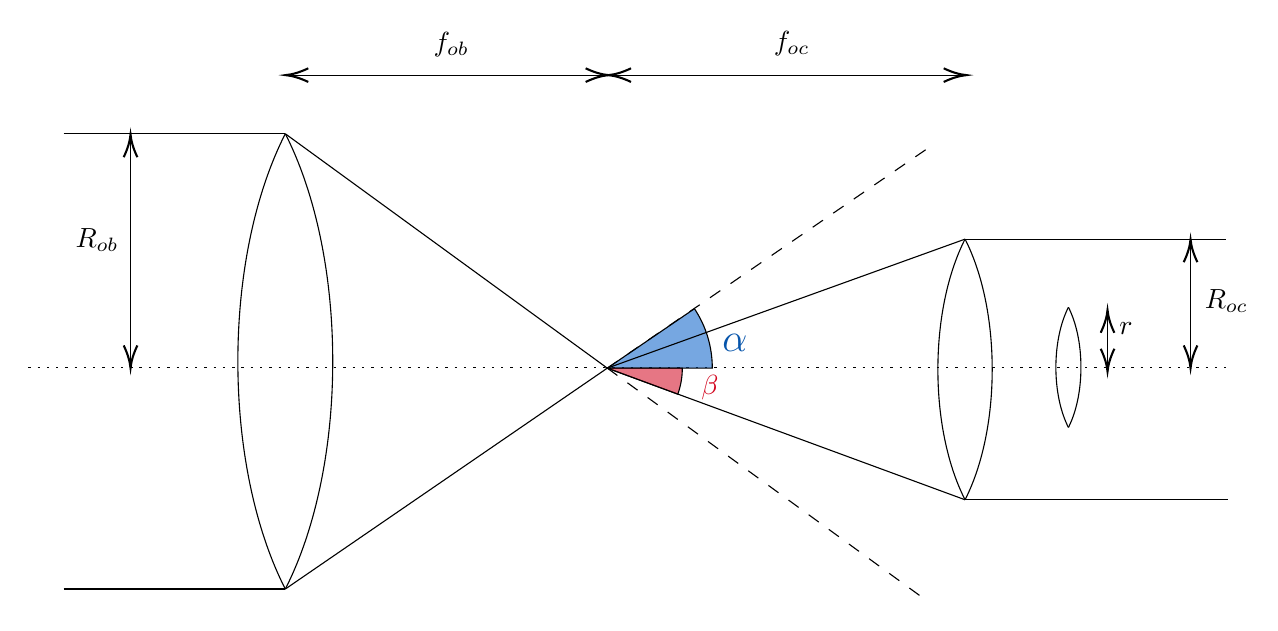
\begin{tikzpicture}[x=0.75pt,y=0.75pt,yscale=-1,xscale=1]
%uncomment if require: \path (0,408); %set diagram left start at 0, and has height of 408

%Shape: Arc [id:dp15226634774792847] 
\draw  [draw opacity=0] (193.86,299.1) .. controls (179.77,271.47) and (171,232.55) .. (171,189.42) .. controls (171,146.3) and (179.77,107.37) .. (193.86,79.75) -- (245,189.42) -- cycle ; \draw   (193.86,299.1) .. controls (179.77,271.47) and (171,232.55) .. (171,189.42) .. controls (171,146.3) and (179.77,107.37) .. (193.86,79.75) ;  
%Shape: Arc [id:dp3199034444063049] 
\draw  [draw opacity=0] (193.86,79.75) .. controls (207.94,107.37) and (216.71,146.3) .. (216.71,189.42) .. controls (216.71,232.55) and (207.94,271.47) .. (193.86,299.1) -- (142.71,189.42) -- cycle ; \draw   (193.86,79.75) .. controls (207.94,107.37) and (216.71,146.3) .. (216.71,189.42) .. controls (216.71,232.55) and (207.94,271.47) .. (193.86,299.1) ;  
%Shape: Arc [id:dp6485254730701198] 
\draw  [draw opacity=0] (521.36,256.09) .. controls (513.29,240.27) and (508.27,217.99) .. (508.27,193.3) .. controls (508.27,168.61) and (513.29,146.32) .. (521.36,130.51) -- (550.64,193.3) -- cycle ; \draw   (521.36,256.09) .. controls (513.29,240.27) and (508.27,217.99) .. (508.27,193.3) .. controls (508.27,168.61) and (513.29,146.32) .. (521.36,130.51) ;  
%Shape: Arc [id:dp8159178562980318] 
\draw  [draw opacity=0] (521.36,130.51) .. controls (529.42,146.32) and (534.44,168.61) .. (534.44,193.3) .. controls (534.44,217.99) and (529.42,240.27) .. (521.36,256.09) -- (492.08,193.3) -- cycle ; \draw   (521.36,130.51) .. controls (529.42,146.32) and (534.44,168.61) .. (534.44,193.3) .. controls (534.44,217.99) and (529.42,240.27) .. (521.36,256.09) ;  
%Straight Lines [id:da2926698443839979] 
\draw  [dash pattern={on 0.84pt off 2.51pt}]  (70,192.27) -- (647.8,192.27) ;
%Straight Lines [id:da5558392846913618] 
\draw    (87,79.75) -- (193.86,79.75) ;
%Straight Lines [id:da6946986660163219] 
\draw    (87,299.1) -- (193.86,299.1) ;
%Straight Lines [id:da8472421076244225] 
\draw    (521.36,130.51) -- (647,130.51) ;
%Straight Lines [id:da17632075659520474] 
\draw    (521.36,256.09) -- (648.2,256.09) ;
%Straight Lines [id:da7968584571366701] 
\draw    (193.86,79.75) -- (349,192.67) ;
%Straight Lines [id:da37990553982592834] 
\draw  [dash pattern={on 4.5pt off 4.5pt}]  (349,192.67) -- (504.14,305.6) ;
%Straight Lines [id:da03767007078975415] 
\draw    (193.86,299.1) -- (349,192.67) ;
%Straight Lines [id:da10833854217864869] 
\draw  [dash pattern={on 4.5pt off 4.5pt}]  (349,192.67) -- (504.14,86.25) ;
%Straight Lines [id:da0878345007392134] 
\draw    (349,192.67) -- (521.36,256.09) ;
%Shape: Pie [id:dp2692707301081927] 
\draw  [fill={rgb, 255:red, 6; green, 95; blue, 200 }  ,fill opacity=0.55 ] (390.98,164.03) .. controls (396.41,172.21) and (399.58,182.07) .. (399.58,192.67) -- (349,192.67) -- cycle ;
%Straight Lines [id:da6003327815384676] 
\draw    (349,192.67) -- (521.36,130.51) ;
%Shape: Pie [id:dp4636891283950564] 
\draw  [fill={rgb, 255:red, 208; green, 2; blue, 27 }  ,fill opacity=0.54 ] (385.13,192.67) .. controls (385.13,192.67) and (385.13,192.67) .. (385.13,192.67) .. controls (385.13,197.08) and (384.37,201.3) .. (382.96,205.21) -- (349,192.67) -- cycle ;
%Straight Lines [id:da527727020353399] 
\draw    (119.29,82.1) -- (119.29,190.67) ;
\draw [shift={(119.29,192.67)}, rotate = 270] [color={rgb, 255:red, 0; green, 0; blue, 0 }  ][line width=0.75]    (10.93,-3.29) .. controls (6.95,-1.4) and (3.31,-0.3) .. (0,0) .. controls (3.31,0.3) and (6.95,1.4) .. (10.93,3.29)   ;
\draw [shift={(119.29,80.1)}, rotate = 90] [color={rgb, 255:red, 0; green, 0; blue, 0 }  ][line width=0.75]    (10.93,-3.29) .. controls (6.95,-1.4) and (3.31,-0.3) .. (0,0) .. controls (3.31,0.3) and (6.95,1.4) .. (10.93,3.29)   ;
%Shape: Arc [id:dp25410735917200733] 
\draw  [draw opacity=0] (571.16,221.25) .. controls (567.44,213.95) and (565.12,203.67) .. (565.12,192.29) .. controls (565.12,180.9) and (567.44,170.62) .. (571.16,163.33) -- (584.66,192.29) -- cycle ; \draw   (571.16,221.25) .. controls (567.44,213.95) and (565.12,203.67) .. (565.12,192.29) .. controls (565.12,180.9) and (567.44,170.62) .. (571.16,163.33) ;  
%Shape: Arc [id:dp6017434664154637] 
\draw  [draw opacity=0] (571.16,163.33) .. controls (574.88,170.62) and (577.19,180.9) .. (577.19,192.29) .. controls (577.19,203.67) and (574.88,213.95) .. (571.16,221.25) -- (557.65,192.29) -- cycle ; \draw   (571.16,163.33) .. controls (574.88,170.62) and (577.19,180.9) .. (577.19,192.29) .. controls (577.19,203.67) and (574.88,213.95) .. (571.16,221.25) ;  
%Straight Lines [id:da49119391009921043] 
\draw    (590,166.68) -- (590,192.28) ;
\draw [shift={(590,194.28)}, rotate = 270] [color={rgb, 255:red, 0; green, 0; blue, 0 }  ][line width=0.75]    (10.93,-3.29) .. controls (6.95,-1.4) and (3.31,-0.3) .. (0,0) .. controls (3.31,0.3) and (6.95,1.4) .. (10.93,3.29)   ;
\draw [shift={(590,164.68)}, rotate = 90] [color={rgb, 255:red, 0; green, 0; blue, 0 }  ][line width=0.75]    (10.93,-3.29) .. controls (6.95,-1.4) and (3.31,-0.3) .. (0,0) .. controls (3.31,0.3) and (6.95,1.4) .. (10.93,3.29)   ;
%Straight Lines [id:da09089919412515335] 
\draw    (630,132.68) -- (630,190.68) ;
\draw [shift={(630,192.68)}, rotate = 270] [color={rgb, 255:red, 0; green, 0; blue, 0 }  ][line width=0.75]    (10.93,-3.29) .. controls (6.95,-1.4) and (3.31,-0.3) .. (0,0) .. controls (3.31,0.3) and (6.95,1.4) .. (10.93,3.29)   ;
\draw [shift={(630,130.68)}, rotate = 90] [color={rgb, 255:red, 0; green, 0; blue, 0 }  ][line width=0.75]    (10.93,-3.29) .. controls (6.95,-1.4) and (3.31,-0.3) .. (0,0) .. controls (3.31,0.3) and (6.95,1.4) .. (10.93,3.29)   ;
%Straight Lines [id:da9569825686529223] 
\draw    (196,51.5) -- (347.5,51.5) ;
\draw [shift={(349.5,51.5)}, rotate = 180] [color={rgb, 255:red, 0; green, 0; blue, 0 }  ][line width=0.75]    (10.93,-3.29) .. controls (6.95,-1.4) and (3.31,-0.3) .. (0,0) .. controls (3.31,0.3) and (6.95,1.4) .. (10.93,3.29)   ;
\draw [shift={(194,51.5)}, rotate = 0] [color={rgb, 255:red, 0; green, 0; blue, 0 }  ][line width=0.75]    (10.93,-3.29) .. controls (6.95,-1.4) and (3.31,-0.3) .. (0,0) .. controls (3.31,0.3) and (6.95,1.4) .. (10.93,3.29)   ;
%Straight Lines [id:da9088169706392342] 
\draw    (351.5,51.5) -- (520,51.5) ;
\draw [shift={(522,51.5)}, rotate = 180] [color={rgb, 255:red, 0; green, 0; blue, 0 }  ][line width=0.75]    (10.93,-3.29) .. controls (6.95,-1.4) and (3.31,-0.3) .. (0,0) .. controls (3.31,0.3) and (6.95,1.4) .. (10.93,3.29)   ;
\draw [shift={(349.5,51.5)}, rotate = 0] [color={rgb, 255:red, 0; green, 0; blue, 0 }  ][line width=0.75]    (10.93,-3.29) .. controls (6.95,-1.4) and (3.31,-0.3) .. (0,0) .. controls (3.31,0.3) and (6.95,1.4) .. (10.93,3.29)   ;

% Text Node
\draw (403.2,175) node [anchor=north west][inner sep=0.75pt]  [font=\Large,color={rgb, 255:red, 7; green, 85; blue, 171 }  ,opacity=1 ]  {$\alpha$};
% Text Node
\draw (393,194.68) node [anchor=north west][inner sep=0.75pt]  [font=\normalsize]  {$\textcolor[rgb]{0.82,0.01,0.11}{\beta }$};
% Text Node
\draw (91.54,123.96) node [anchor=north west][inner sep=0.75pt]    {$R_{ob}$};
% Text Node
\draw (594.4,169.28) node [anchor=north west][inner sep=0.75pt]    {$r$};
% Text Node
\draw (635.6,153.48) node [anchor=north west][inner sep=0.75pt]    {$R_{oc}$};
% Text Node
\draw (264,29.4) node [anchor=north west][inner sep=0.75pt]    {$f_{ob}$};
% Text Node
\draw (428,28.9) node [anchor=north west][inner sep=0.75pt]    {$f_{oc}$};


\end{tikzpicture}
	
        \caption{Representation of the fraction of light that effectively passes through the two lenses of Nill's refracting telescope}
        \label{fig:refrat}
    \end{figure}	

	
	We will perform the analysis by comparing the flux that reaches the observer's eye with the actual flux emitted by the celestial object. We will call the original flux $F$ and the limiting flux for human vision $F_0$ (the smallest flux at which something can be observed). Note that the power that effectively enters the telescope is $P=F\pi R_{ob}^2(1-\epsilon)$ ($1-\epsilon$ because this corresponds to the transmitted part—the complement of the absorbed part). This power is concentrated at the focal point of the lenses and then spreads out toward the eyepiece. Note that since $\dfrac{R_{oc}}{f_{oc}} < \dfrac{R_{ob}}{f_{ob}}$, we have $\tan{(\beta)} < \tan{(\alpha)}$, which implies $\beta < \alpha$, and therefore not all the power passes through the eyepiece.
	
	The fraction that passes depends on the solid angle corresponding to this aperture. Thus:
	
	$$\frac{P_{oc}}{P_{total}}=\frac{\Omega(\beta)}{\Omega(\alpha)}$$
	
	As discussed in other problems, we know that $\Omega(\theta)=2\pi (1-\cos{(\theta)})$, so the power that passes through the eyepiece is:
	
	$$P_{oc}=F \pi R_{ob}^2(1-\epsilon)^2\frac{1-\cos{(\beta)}}{1-\cos{(\alpha)}}$$
	
	Notice that we multiply again by $1-\epsilon$ to take into account only the transmitted part. Note that even so, not all the radiation (which exits parallel to the axis) reaches the observer's eye, since the diameter of the pupil is smaller than the diameter of the eyepiece. Thus, the part that effectively enters is proportional to the area:
	
	$$\frac{P_{olho}}{P_{oc}}=\frac{\pi r^2}{\pi R_{oc}^2}$$
	
	Thus:
	
	$$P_{olho}=F \pi \left(\frac{R_{ob}}{R_{oc}}\right)^2(1-\epsilon)^2\frac{1-\cos{(\beta)}}{1-\cos{(\alpha)}}r^2$$
	
	The flux is the power divided by the area $(\pi r^2)$:
	
	$$F_{olho}=F \left(\frac{R_{ob}}{R_{oc}}\right)^2(1-\epsilon)^2\frac{1-\cos{(\beta)}}{1-\cos{(\alpha)}}$$
	
	It is interesting that in this case the dimensions of the pupil are irrelevant, as long as $r<R_{oc}$! In the limiting case, we set $F_{olho}=F_0$, thus:
	
	$$F=F_0\left(\frac{R_{oc}}{R_{ob}}\right)^2(1-\epsilon)^{-2}\frac{1-\cos{(\alpha)}}{1-\cos{(\beta)}}$$
	
	Since $m_0=6=-2.5\log{(F_0/F_r)}$ (with $F_r$ being the reference flux), we can find that:
	
	$$m_{lim}=-2.5\log{\left [  \frac{F_0}{F_r}\left(\frac{R_{oc}}{R_{ob}}\right)^2(1-\epsilon)^{-2}\frac{1-\cos{(\alpha)}}{1-\cos{(\beta)}} \right ] }$$
	
	Simplifying and rearranging, we obtain:
	
	$$m_{lim}=m_0+5\log{ \left [ \frac{R_{ob}}{R_{oc}}(1-\epsilon) \sqrt{\frac{1-\cos{(\beta)}}{1-\cos{(\alpha)}}} \right ] }$$
	
	Substituting the values:
	
	$$m_{lim}=10.02$$
	
	
	\begin{doublespace}
		
		
		\begin{large}
			\textbf{Part B: Reflecting Telescopes}
		\end{large}
		
	\end{doublespace}
	
	\ut{B.1} Choose a point on the ellipse with foci $A$ and $B$ and draw the tangent that passes through this point. A ray of light, upon striking the mirror, would behave as if it were incident on a plane mirror coinciding with the tangent line, so we want to prove that the angles $\alpha$ and $\beta$ in Figure \ref{fig:elipsereflex}.


	\begin{figure}[htpb]
	    \centering
	    

\tikzset{every picture/.style={line width=0.75pt}} %set default line width to 0.75pt        

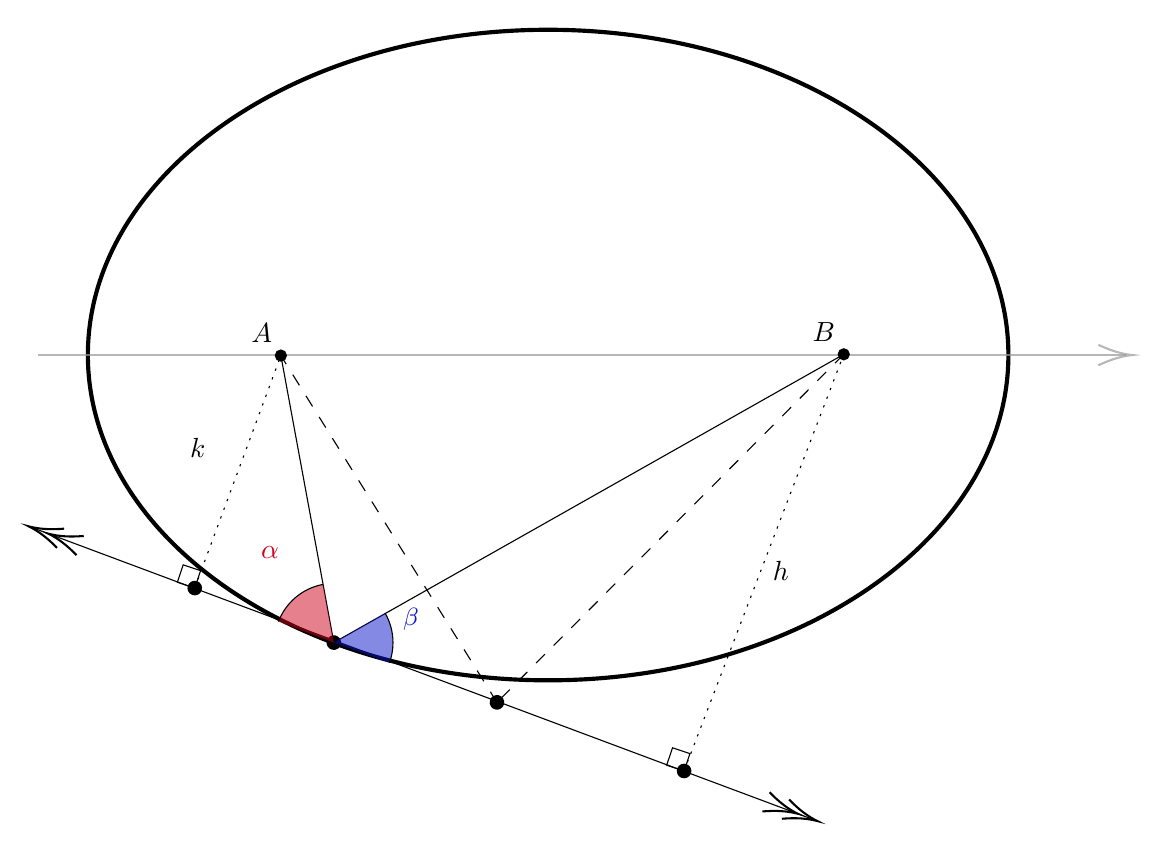
\begin{tikzpicture}[x=0.75pt,y=0.75pt,yscale=-1.5,xscale=1.5]
%uncomment if require: \path (0,542); %set diagram left start at 0, and has height of 542

%Shape: Ellipse [id:dp8979721006541848] 
\draw  [color={rgb, 255:red, 0; green, 0; blue, 0 }  ,draw opacity=1 ][line width=1.5]  (148,234.32) .. controls (148,176.62) and (214.19,129.84) .. (295.83,129.84) .. controls (377.48,129.84) and (443.67,176.62) .. (443.67,234.32) .. controls (443.67,292.02) and (377.48,338.8) .. (295.83,338.8) .. controls (214.19,338.8) and (148,292.02) .. (148,234.32) -- cycle ;
%Straight Lines [id:da5987369599518098] 
\draw [color={rgb, 255:red, 155; green, 155; blue, 155 }  ,draw opacity=0.72 ][line width=0.75]    (132,234.32) -- (481.5,234.32) ;
\draw [shift={(483.5,234.32)}, rotate = 180] [color={rgb, 255:red, 155; green, 155; blue, 155 }  ,draw opacity=0.72 ][line width=0.75]    (10.93,-3.29) .. controls (6.95,-1.4) and (3.31,-0.3) .. (0,0) .. controls (3.31,0.3) and (6.95,1.4) .. (10.93,3.29)   ;
%Shape: Circle [id:dp3527055407446611] 
\draw  [fill={rgb, 255:red, 0; green, 0; blue, 0 }  ,fill opacity=1 ] (208.2,234.49) .. controls (208.2,233.5) and (209,232.7) .. (209.99,232.7) .. controls (210.97,232.7) and (211.77,233.5) .. (211.77,234.49) .. controls (211.77,235.47) and (210.97,236.27) .. (209.99,236.27) .. controls (209,236.27) and (208.2,235.47) .. (208.2,234.49) -- cycle ;
%Shape: Circle [id:dp8770097356475901] 
\draw  [fill={rgb, 255:red, 0; green, 0; blue, 0 }  ,fill opacity=1 ] (389,234.09) .. controls (389,233.1) and (389.8,232.3) .. (390.79,232.3) .. controls (391.77,232.3) and (392.57,233.1) .. (392.57,234.09) .. controls (392.57,235.07) and (391.77,235.87) .. (390.79,235.87) .. controls (389.8,235.87) and (389,235.07) .. (389,234.09) -- cycle ;
%Straight Lines [id:da8011513688052272] 
\draw    (129,289.34) -- (382.33,384.01) ;
\draw [shift={(382.33,384.01)}, rotate = 200.49] [color={rgb, 255:red, 0; green, 0; blue, 0 }  ][line width=0.75]    (17.64,-3.29) .. controls (13.66,-1.4) and (10.02,-0.3) .. (6.71,0) .. controls (10.02,0.3) and (13.66,1.4) .. (17.64,3.29)(10.93,-3.29) .. controls (6.95,-1.4) and (3.31,-0.3) .. (0,0) .. controls (3.31,0.3) and (6.95,1.4) .. (10.93,3.29)   ;
\draw [shift={(129,289.34)}, rotate = 20.49] [color={rgb, 255:red, 0; green, 0; blue, 0 }  ][line width=0.75]    (17.64,-3.29) .. controls (13.66,-1.4) and (10.02,-0.3) .. (6.71,0) .. controls (10.02,0.3) and (13.66,1.4) .. (17.64,3.29)(10.93,-3.29) .. controls (6.95,-1.4) and (3.31,-0.3) .. (0,0) .. controls (3.31,0.3) and (6.95,1.4) .. (10.93,3.29)   ;
%Straight Lines [id:da38204483076300577] 
\draw  [dash pattern={on 0.84pt off 2.51pt}]  (182.33,309.17) -- (209.99,234.49) ;
\draw [shift={(182.33,309.17)}, rotate = 290.32] [color={rgb, 255:red, 0; green, 0; blue, 0 }  ][fill={rgb, 255:red, 0; green, 0; blue, 0 }  ][line width=0.75]      (0, 0) circle [x radius= 2.01, y radius= 2.01]   ;
%Shape: Square [id:dp8345305118777975] 
\draw   (178.62,301.71) -- (184.21,303.59) -- (182.33,309.17) -- (176.75,307.3) -- cycle ;
%Straight Lines [id:da3036688498162936] 
\draw  [dash pattern={on 0.84pt off 2.51pt}]  (339.5,367.92) -- (390.79,234.09) ;
\draw [shift={(339.5,367.92)}, rotate = 290.97] [color={rgb, 255:red, 0; green, 0; blue, 0 }  ][fill={rgb, 255:red, 0; green, 0; blue, 0 }  ][line width=0.75]      (0, 0) circle [x radius= 2.01, y radius= 2.01]   ;
%Shape: Square [id:dp5365954794391563] 
\draw   (335.79,360.46) -- (341.38,362.34) -- (339.5,367.92) -- (333.91,366.05) -- cycle ;
%Straight Lines [id:da8001871056999452] 
\draw    (227,326.68) -- (209.99,234.49) ;
\draw [shift={(227,326.68)}, rotate = 259.54] [color={rgb, 255:red, 0; green, 0; blue, 0 }  ][fill={rgb, 255:red, 0; green, 0; blue, 0 }  ][line width=0.75]      (0, 0) circle [x radius= 2.01, y radius= 2.01]   ;
%Straight Lines [id:da03249677251103433] 
\draw    (390.79,234.09) -- (227,326.68) ;
%Straight Lines [id:da7799810542592538] 
\draw  [dash pattern={on 4.5pt off 4.5pt}]  (279.4,345.88) -- (209.99,234.49) ;
\draw [shift={(279.4,345.88)}, rotate = 238.07] [color={rgb, 255:red, 0; green, 0; blue, 0 }  ][fill={rgb, 255:red, 0; green, 0; blue, 0 }  ][line width=0.75]      (0, 0) circle [x radius= 2.01, y radius= 2.01]   ;
%Straight Lines [id:da5730666708392338] 
\draw  [dash pattern={on 4.5pt off 4.5pt}]  (390.79,234.09) -- (279.4,345.88) ;
%Shape: Arc [id:dp19044230165471476] 
\draw  [draw opacity=0][fill={rgb, 255:red, 208; green, 2; blue, 27 }  ,fill opacity=0.5 ] (209.23,319.93) .. controls (211.54,313.84) and (216.9,309.25) .. (223.45,308.01) -- (227,326.68) -- cycle ; \draw   (209.23,319.93) .. controls (211.54,313.84) and (216.9,309.25) .. (223.45,308.01) ;  
%Shape: Arc [id:dp9214952410487034] 
\draw  [draw opacity=0][fill={rgb, 255:red, 10; green, 20; blue, 200 }  ,fill opacity=0.5 ] (243.48,317.22) .. controls (245.08,320) and (246,323.23) .. (246,326.68) .. controls (246,328.96) and (245.6,331.14) .. (244.86,333.17) -- (227,326.68) -- cycle ; \draw   (243.48,317.22) .. controls (245.08,320) and (246,323.23) .. (246,326.68) .. controls (246,328.96) and (245.6,331.14) .. (244.86,333.17) ;  

% Text Node
\draw (207.99,231.09) node [anchor=south east] [inner sep=0.75pt]    {$A$};
% Text Node
\draw (388.79,230.69) node [anchor=south east] [inner sep=0.75pt]    {$B$};
% Text Node
\draw (202.8,295.07) node [anchor=north west][inner sep=0.75pt]  [color={rgb, 255:red, 208; green, 2; blue, 27 }  ,opacity=1 ]  {$\alpha $};
% Text Node
\draw (248.4,314.67) node [anchor=north west][inner sep=0.75pt]  [font=\small,color={rgb, 255:red, 10; green, 20; blue, 200 }  ,opacity=1 ]  {$\beta $};
% Text Node
\draw (180,260.07) node [anchor=north west][inner sep=0.75pt]    {$k$};
% Text Node
\draw (367.2,299.67) node [anchor=north west][inner sep=0.75pt]    {$h$};


\end{tikzpicture}
	
	    \caption{Geometric relation of the points of the ellipse with the tangent line at a generic point}
	    \label{fig:elipsereflex}
	\end{figure}


	
	Draw also a segment perpendicular to the tangent that starts from each focus (segments $K$ and $H$). Note that the sum of the distances from the point that defines the tangent to the two foci is equal, by definition, to the major axis of the ellipse $2a$; however, note another important factor: this is the point on the tangent line that minimizes this sum (just look at the figure).
	
	In this way, we want to prove that for this point of minimum $\alpha=\beta$. This distance from the point to the foci is given by:
	
	$$d=\frac{K}{\sin{(\alpha)}}+\frac{H}{\sin{(\beta)}}$$
	
	For $d$ to be minimum, it suffices to differentiate and set it equal to zero:
	
	$$\frac{K}{\sin^2{(\alpha)}}\cos{(\alpha)}d\alpha=-\frac{H}{\sin^2{(\beta)}}\cos{(\beta)}d\beta$$
	
	Note that the sum of the distances from a point to the orthogonal projections of $A$ and $B$ onto the tangent line is constant for points within this interval:
	
	
	$$\frac{K}{\tan{(\alpha)}}+\frac{H}{\tan{(\beta)}}=\text{constant}$$
	
	Thus:
	
	$$\frac{K}{\sin^2{(\alpha)}}d\alpha=-\frac{H}{\sin^2{(\beta)}}d\beta$$
	
	Which implies that $\cos{(\alpha)}=\cos{(\beta)}$, which, under the conditions of the analysis, means that $\alpha=\beta$. Thus, the relation that the angle of incidence is equal to the angle of reflection is satisfied, and therefore each ray that originates from one of the foci strikes the ellipse and goes to the other focus.
	
	\ut{B.2} We can prove this item in isolation using analytic geometry and going through the calculations (writing the equation of the tangent line, finding the relations between the angles from trigonometric relations and derivatives, etc.), or even by plane geometry, starting from the definition of a parabola and studying the points that belong to the tangent line and noting that the only point that is at equal distance from the directrix and the focus (similar to what we did in the proof for the ellipse). However, we will do something different!
	
	Recall that ellipses have eccentricity $0 \le e < 1$. Note that $e \ne 1$, but we can fix one focus at the origin, for example, and let $e \rightarrow 1$ (that is, $e$ tends to $1$), which would make the ellipse in question approach arbitrarily close to a parabola. Also note that as $e \rightarrow 1$, the unfixed focus tends to infinity, so a ray of light coming from it would tend to come almost parallel to the axis of the ellipse and converge at the fixed focus, which proves\footnote{Our mathematical colleagues were probably quite dissatisfied with this non-rigorous "proof", but in this case practicality spoke louder than rigor!} the stated property!
	
	\ut{B.3} We will follow a line of reasoning similar to that of the proof for the ellipse\footnote{If you stop to pay attention, the difference between the definition of a hyperbola and an ellipse is just a sign: while one involves the sum of the distances, the other involves the difference of the distances.}, for this, consider the following scheme, where a ray of light "aims" at focus $A$ and is reflected at point $D$, as shown in Figure \ref{fig:tele7}:


	\begin{figure}[htpb]
	    \centering
	    

\tikzset{every picture/.style={line width=0.75pt}} %set default line width to 0.75pt        

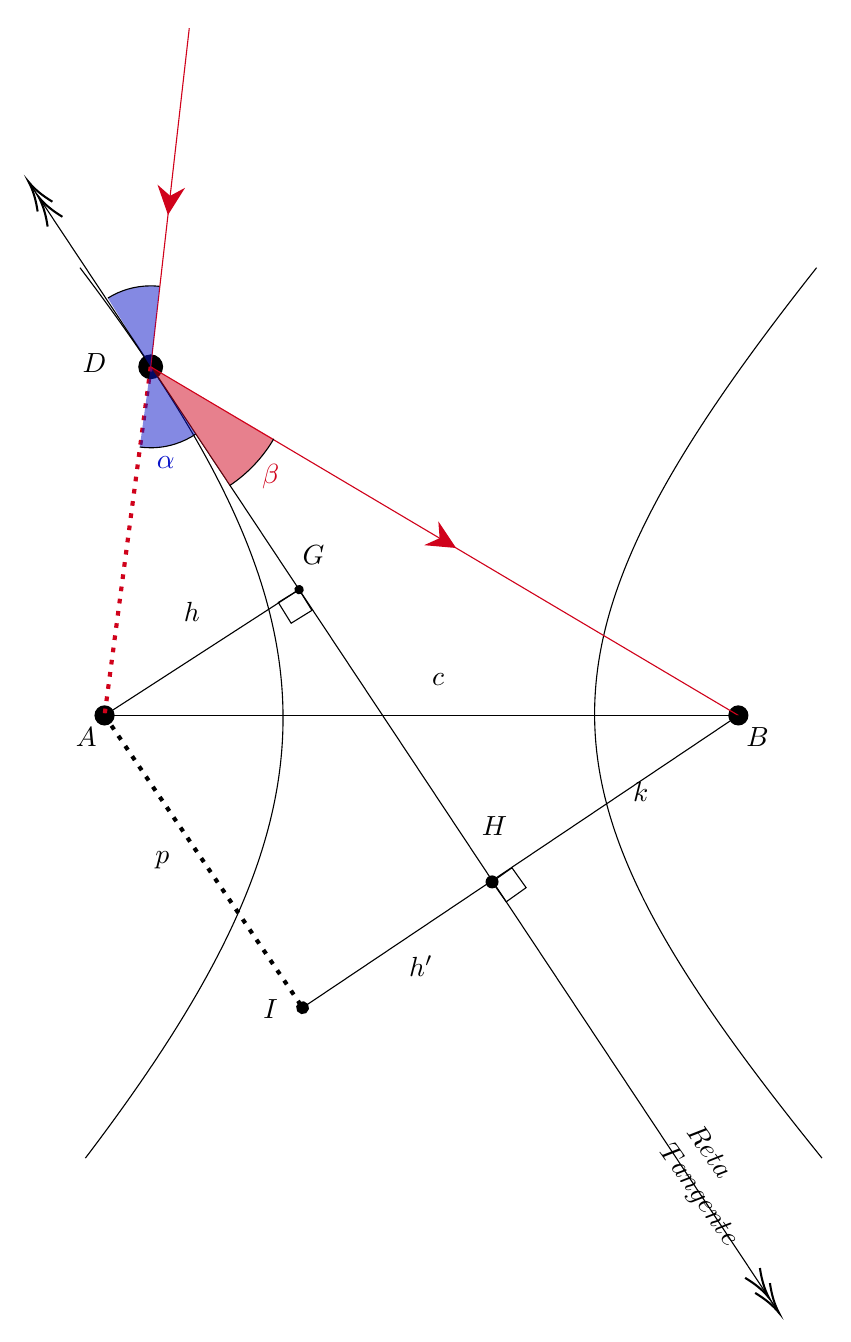
\begin{tikzpicture}[x=0.75pt,y=0.75pt,yscale=-1.3,xscale=1.3]
%uncomment if require: \path (0,643); %set diagram left start at 0, and has height of 643

%Curve Lines [id:da0922538905744319] 
\draw    (275,218.17) .. controls (375,350.17) and (375,419.17) .. (277,548.17) ;
%Curve Lines [id:da21181179276379836] 
\draw    (548,218.17) .. controls (435,361.17) and (441,413.17) .. (550,548.17) ;
%Straight Lines [id:da9759862466504334] 
\draw    (284.1,384.1) -- (519,384.1) ;
\draw [shift={(519,384.1)}, rotate = 0] [color={rgb, 255:red, 0; green, 0; blue, 0 }  ][fill={rgb, 255:red, 0; green, 0; blue, 0 }  ][line width=0.75]      (0, 0) circle [x radius= 3.35, y radius= 3.35]   ;
\draw [shift={(284.1,384.1)}, rotate = 0] [color={rgb, 255:red, 0; green, 0; blue, 0 }  ][fill={rgb, 255:red, 0; green, 0; blue, 0 }  ][line width=0.75]      (0, 0) circle [x radius= 3.35, y radius= 3.35]   ;
%Shape: Circle [id:dp22662378462429045] 
\draw  [fill={rgb, 255:red, 0; green, 0; blue, 0 }  ,fill opacity=1 ] (296.8,254.9) .. controls (296.8,252.47) and (298.77,250.5) .. (301.2,250.5) .. controls (303.63,250.5) and (305.6,252.47) .. (305.6,254.9) .. controls (305.6,257.33) and (303.63,259.3) .. (301.2,259.3) .. controls (298.77,259.3) and (296.8,257.33) .. (296.8,254.9) -- cycle ;
%Straight Lines [id:da5352812127954605] 
\draw    (256,186.42) -- (534,605.42) ;
\draw [shift={(534,605.42)}, rotate = 236.44] [color={rgb, 255:red, 0; green, 0; blue, 0 }  ][line width=0.75]    (17.64,-3.29) .. controls (13.66,-1.4) and (10.02,-0.3) .. (6.71,0) .. controls (10.02,0.3) and (13.66,1.4) .. (17.64,3.29)(10.93,-3.29) .. controls (6.95,-1.4) and (3.31,-0.3) .. (0,0) .. controls (3.31,0.3) and (6.95,1.4) .. (10.93,3.29)   ;
\draw [shift={(256,186.42)}, rotate = 56.44] [color={rgb, 255:red, 0; green, 0; blue, 0 }  ][line width=0.75]    (17.64,-3.29) .. controls (13.66,-1.4) and (10.02,-0.3) .. (6.71,0) .. controls (10.02,0.3) and (13.66,1.4) .. (17.64,3.29)(10.93,-3.29) .. controls (6.95,-1.4) and (3.31,-0.3) .. (0,0) .. controls (3.31,0.3) and (6.95,1.4) .. (10.93,3.29)   ;
%Straight Lines [id:da30830459830846313] 
\draw [color={rgb, 255:red, 208; green, 2; blue, 27 }  ,draw opacity=1 ][line width=1.5]  [dash pattern={on 1.69pt off 2.76pt}]  (301.2,254.9) -- (284.1,384.1) ;
%Straight Lines [id:da20460744432028166] 
\draw [color={rgb, 255:red, 208; green, 2; blue, 27 }  ,draw opacity=1 ]   (301.2,254.9) -- (519,384.1) ;
\draw [shift={(414.4,322.05)}, rotate = 210.68] [fill={rgb, 255:red, 208; green, 2; blue, 27 }  ,fill opacity=1 ][line width=0.08]  [draw opacity=0] (10.72,-5.15) -- (0,0) -- (10.72,5.15) -- (7.12,0) -- cycle    ;
%Straight Lines [id:da17552819998896774] 
\draw [color={rgb, 255:red, 208; green, 2; blue, 27 }  ,draw opacity=1 ]   (301.2,254.9) -- (315.5,129.42) ;
\draw [shift={(307.62,198.62)}, rotate = 276.5] [fill={rgb, 255:red, 208; green, 2; blue, 27 }  ,fill opacity=1 ][line width=0.08]  [draw opacity=0] (10.72,-5.15) -- (0,0) -- (10.72,5.15) -- (7.12,0) -- cycle    ;
%Straight Lines [id:da6676254497457772] 
\draw    (284.1,384.1) -- (356.2,337.48) ;
\draw [shift={(356.2,337.48)}, rotate = 327.11] [color={rgb, 255:red, 0; green, 0; blue, 0 }  ][fill={rgb, 255:red, 0; green, 0; blue, 0 }  ][line width=0.75]      (0, 0) circle [x radius= 1.34, y radius= 1.34]   ;
%Shape: Square [id:dp3567637297226198] 
\draw   (348.5,342.23) -- (356.2,337.48) -- (360.96,345.17) -- (353.26,349.93) -- cycle ;
%Straight Lines [id:da6593293553091812] 
\draw    (357.5,492.42) -- (519,384.1) ;
\draw [shift={(357.5,492.42)}, rotate = 326.15] [color={rgb, 255:red, 0; green, 0; blue, 0 }  ][fill={rgb, 255:red, 0; green, 0; blue, 0 }  ][line width=0.75]      (0, 0) circle [x radius= 2.01, y radius= 2.01]   ;
%Shape: Square [id:dp8527223072248471] 
\draw   (427.72,445.8) -- (435.09,440.56) -- (440.34,447.93) -- (432.97,453.18) -- cycle ;
%Straight Lines [id:da3000572837618136] 
\draw [line width=1.5]  [dash pattern={on 1.69pt off 2.76pt}]  (284.1,384.1) -- (357.5,492.42) ;
%Shape: Circle [id:dp4895920223737915] 
\draw  [fill={rgb, 255:red, 0; green, 0; blue, 0 }  ,fill opacity=1 ] (425.52,445.8) .. controls (425.52,444.59) and (426.51,443.6) .. (427.72,443.6) .. controls (428.93,443.6) and (429.92,444.59) .. (429.92,445.8) .. controls (429.92,447.02) and (428.93,448) .. (427.72,448) .. controls (426.51,448) and (425.52,447.02) .. (425.52,445.8) -- cycle ;
%Shape: Arc [id:dp05094588203923878] 
\draw  [draw opacity=0][fill={rgb, 255:red, 10; green, 20; blue, 200 }  ,fill opacity=0.5 ] (317.89,279.84) .. controls (313.12,283.04) and (307.38,284.9) .. (301.2,284.9) .. controls (299.83,284.9) and (298.48,284.81) .. (297.15,284.63) -- (301.2,254.9) -- cycle ; \draw  [color={rgb, 255:red, 0; green, 0; blue, 0 }  ,draw opacity=1 ] (317.89,279.84) .. controls (313.12,283.04) and (307.38,284.9) .. (301.2,284.9) .. controls (299.83,284.9) and (298.48,284.81) .. (297.15,284.63) ;  
%Shape: Arc [id:dp7936611916939003] 
\draw  [draw opacity=0][fill={rgb, 255:red, 10; green, 20; blue, 200 }  ,fill opacity=0.5 ] (285.33,229.44) .. controls (289.93,226.56) and (295.37,224.9) .. (301.2,224.9) .. controls (302.3,224.9) and (303.39,224.96) .. (304.46,225.08) -- (301.2,254.9) -- cycle ; \draw  [color={rgb, 255:red, 0; green, 0; blue, 0 }  ,draw opacity=1 ] (285.33,229.44) .. controls (289.93,226.56) and (295.37,224.9) .. (301.2,224.9) .. controls (302.3,224.9) and (303.39,224.96) .. (304.46,225.08) ;  
%Shape: Arc [id:dp6220595950879206] 
\draw  [draw opacity=0][fill={rgb, 255:red, 208; green, 2; blue, 27 }  ,fill opacity=0.5 ] (346.81,281.62) .. controls (342.75,288.54) and (337.16,294.45) .. (330.5,298.89) -- (301.2,254.9) -- cycle ; \draw  [color={rgb, 255:red, 0; green, 0; blue, 0 }  ,draw opacity=1 ] (346.81,281.62) .. controls (342.75,288.54) and (337.16,294.45) .. (330.5,298.89) ;  

% Text Node
\draw (282.1,387.5) node [anchor=north east] [inner sep=0.75pt]    {$A$};
% Text Node
\draw (521,387.5) node [anchor=north west][inner sep=0.75pt]    {$B$};
% Text Node
\draw (275,249.07) node [anchor=north west][inner sep=0.75pt]    {$D$};
% Text Node
\draw (396,472.07) node [anchor=north west][inner sep=0.75pt]    {$h'$};
% Text Node
\draw (312.5,341.07) node [anchor=north west][inner sep=0.75pt]    {$h$};
% Text Node
\draw (356.5,320.07) node [anchor=north west][inner sep=0.75pt]    {$G$};
% Text Node
\draw (404.5,367.57) node [anchor=north west][inner sep=0.75pt]    {$c$};
% Text Node
\draw (423,420.57) node [anchor=north west][inner sep=0.75pt]    {$H$};
% Text Node
\draw (479,408.07) node [anchor=north west][inner sep=0.75pt]    {$k$};
% Text Node
\draw (302.5,287.07) node [anchor=north west][inner sep=0.75pt]  [color={rgb, 255:red, 10; green, 20; blue, 200 }  ,opacity=1 ]  {$\alpha $};
% Text Node
\draw (341.5,290.07) node [anchor=north west][inner sep=0.75pt]  [color={rgb, 255:red, 208; green, 2; blue, 27 }  ,opacity=1 ]  {$\beta $};
% Text Node
\draw (302,433.73) node [anchor=north west][inner sep=0.75pt]    {$p$};
% Text Node
\draw (342,488.4) node [anchor=north west][inner sep=0.75pt]    {$I$};
% Text Node
\draw (503.79,528.09) node [anchor=north west][inner sep=0.75pt]  [rotate=-54.58]  {$ \begin{array}{l}
Reta\\
Tangente
\end{array}$};


\end{tikzpicture}
	
	    \caption{Reflection scheme on the hyperbola}
	    \label{fig:tele7}
	\end{figure}

	
	We wish to prove that the angle $\alpha$—which is vertically opposite to the angle of incidence of the ray (which means they are equal)—is equal to the angle $\beta$ (the angle of reflection), since this would guarantee that this is the path followed by the reflected ray.
	
	In the diagram, the tangent line to the conic at $D$ was drawn and the angles shown were defined, with $A$ and $B$ being the foci of the hyperbola. Note that among all the points on the tangent line, $D$ is the one for which $L=\overline{BD}-\overline{DA}$ is maximum. Proceeding to the relations to be developed, note that:
	
	$$\begin{cases}
		\overline{BD}=\frac{K}{\sin{(\beta)}} \\
		\overline{DA}=\frac{h}{\sin{(\alpha)}} \\
		\overline{IB}=K+h \\
		p=\frac{K}{\tan{(\beta)}}-\frac{h}{\tan{(\alpha)}} \\
	\end{cases}$$
	
	Note that when the point $D$ varies along the tangent, the only quantities that change are the angles and the distances $\overline{DA}$ and $\overline{BD}$. Thus, fortunately, $p$, $K$, $h$, and $c$ remain constant:
	
	$$dp=0=\frac{-K}{\sin^2{(\beta)}}d\beta-\frac{-h}{\sin^2{(\alpha)}}d\alpha$$
	$$\therefore \frac{K}{\sin^2{(\beta)}}=\frac{h}{\sin^2{(\alpha)}}$$
	
	For $L$ to be maximum:
	
	$$dL=0=\frac{-K\cos{(\beta)}}{\sin^2{(\beta)}}d\beta-\frac{-h\cos{(\alpha)}}{\sin^2{(\alpha)}}d\alpha$$
	
	Comparing the two previous equations, we finally find that $\cos{(\alpha)}=\cos{(\beta)}$, which, under the conditions of the problem, implies that $\alpha=\beta$, which guarantees the path of the light ray.
	
	
	\ut{B.4} We know that the primary mirror (parabolic) focuses parallel rays at a focal distance of $h+p$, as shown in the figure; thus $f_p=700 mm$.
	
	
	\textbf{NOTE: Consider Figure \ref{fig:geralfig} below for the solution of the next items}


	\begin{figure}[htpb]
	    \centering
	    

\tikzset{every picture/.style={line width=0.75pt}} %set default line width to 0.75pt        

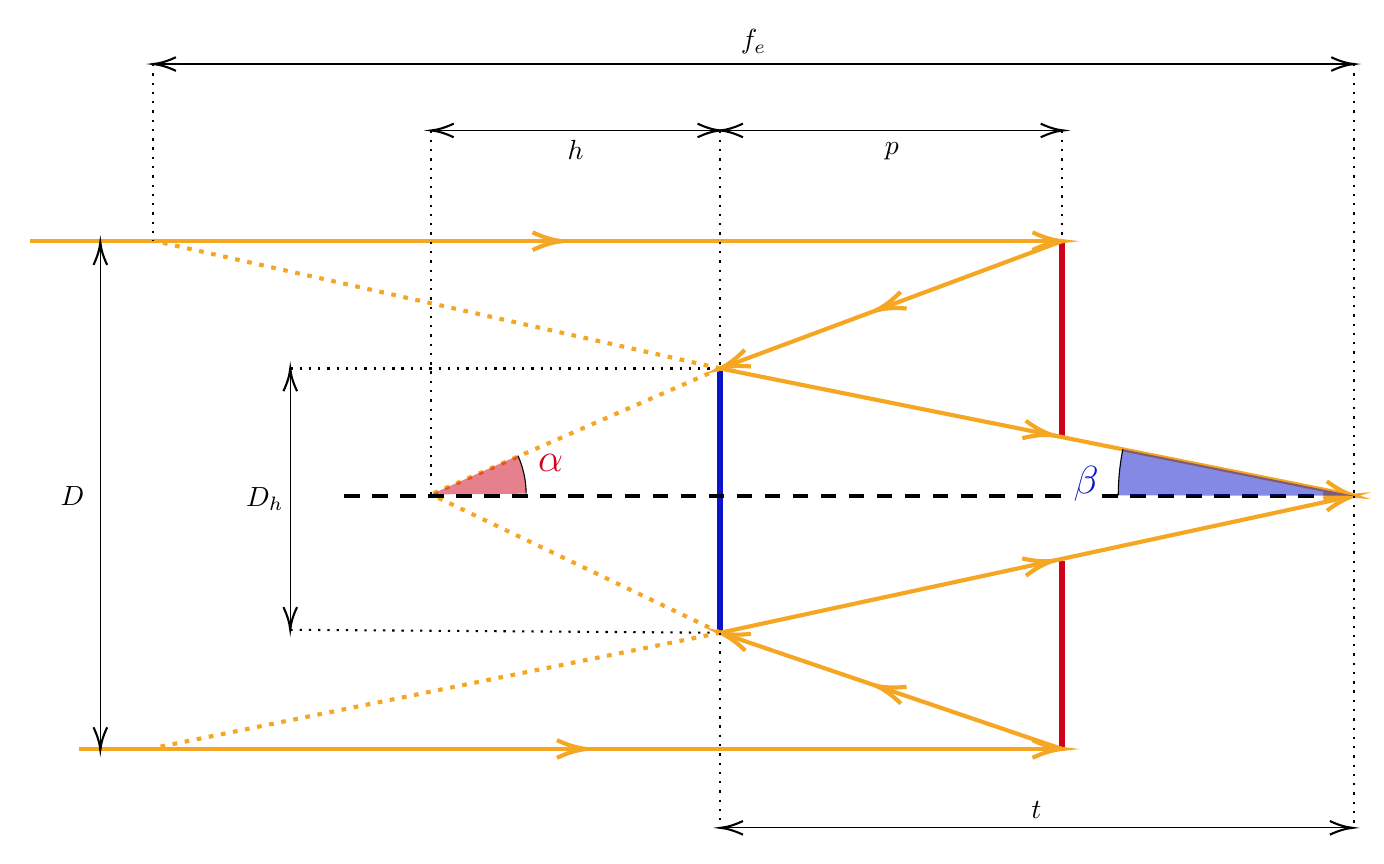
\begin{tikzpicture}[x=0.75pt,y=0.75pt,yscale=-1,xscale=1]
%uncomment if require: \path (0,643); %set diagram left start at 0, and has height of 643

%Straight Lines [id:da19325843126429554] 
\draw [color={rgb, 255:red, 208; green, 2; blue, 27 }  ,draw opacity=1 ][line width=2.25]    (558.33,263.68) -- (558.33,357.68) ;
%Straight Lines [id:da11659437311009069] 
\draw [color={rgb, 255:red, 208; green, 2; blue, 27 }  ,draw opacity=1 ][line width=2.25]    (558.33,417.68) -- (558.33,508.34) ;
%Straight Lines [id:da5649073115870709] 
\draw [color={rgb, 255:red, 10; green, 20; blue, 200 }  ,draw opacity=1 ][line width=2.25]    (393.67,325.01) -- (393.67,452.34) ;
%Straight Lines [id:da544700300665091] 
\draw [color={rgb, 255:red, 0; green, 0; blue, 0 }  ,draw opacity=1 ][line width=1.5]  [dash pattern={on 5.63pt off 4.5pt}]  (577.67,386.34) -- (699,386.34) ;
%Straight Lines [id:da2847065331123977] 
\draw [color={rgb, 255:red, 245; green, 166; blue, 35 }  ,draw opacity=1 ][line width=1.5]    (61,263.68) -- (555.33,263.68) ;
\draw [shift={(558.33,263.68)}, rotate = 180] [color={rgb, 255:red, 245; green, 166; blue, 35 }  ,draw opacity=1 ][line width=1.5]    (14.21,-4.28) .. controls (9.04,-1.82) and (4.3,-0.39) .. (0,0) .. controls (4.3,0.39) and (9.04,1.82) .. (14.21,4.28)   ;
\draw [shift={(317.47,263.68)}, rotate = 180] [color={rgb, 255:red, 245; green, 166; blue, 35 }  ,draw opacity=1 ][line width=1.5]    (14.21,-4.28) .. controls (9.04,-1.82) and (4.3,-0.39) .. (0,0) .. controls (4.3,0.39) and (9.04,1.82) .. (14.21,4.28)   ;
%Straight Lines [id:da6200713098334971] 
\draw [color={rgb, 255:red, 245; green, 166; blue, 35 }  ,draw opacity=1 ][line width=1.5]    (558.33,263.68) -- (396.48,323.96) ;
\draw [shift={(393.67,325.01)}, rotate = 339.57] [color={rgb, 255:red, 245; green, 166; blue, 35 }  ,draw opacity=1 ][line width=1.5]    (14.21,-4.28) .. controls (9.04,-1.82) and (4.3,-0.39) .. (0,0) .. controls (4.3,0.39) and (9.04,1.82) .. (14.21,4.28)   ;
\draw [shift={(468.69,297.07)}, rotate = 339.57] [color={rgb, 255:red, 245; green, 166; blue, 35 }  ,draw opacity=1 ][line width=1.5]    (14.21,-4.28) .. controls (9.04,-1.82) and (4.3,-0.39) .. (0,0) .. controls (4.3,0.39) and (9.04,1.82) .. (14.21,4.28)   ;
%Straight Lines [id:da7464199206603848] 
\draw [color={rgb, 255:red, 245; green, 166; blue, 35 }  ,draw opacity=1 ][line width=1.5]    (393.67,325.01) -- (696.06,385.75) ;
\draw [shift={(699,386.34)}, rotate = 191.36] [color={rgb, 255:red, 245; green, 166; blue, 35 }  ,draw opacity=1 ][line width=1.5]    (14.21,-4.28) .. controls (9.04,-1.82) and (4.3,-0.39) .. (0,0) .. controls (4.3,0.39) and (9.04,1.82) .. (14.21,4.28)   ;
\draw [shift={(553.98,357.21)}, rotate = 191.36] [color={rgb, 255:red, 245; green, 166; blue, 35 }  ,draw opacity=1 ][line width=1.5]    (14.21,-4.28) .. controls (9.04,-1.82) and (4.3,-0.39) .. (0,0) .. controls (4.3,0.39) and (9.04,1.82) .. (14.21,4.28)   ;
%Straight Lines [id:da15421615594891946] 
\draw [color={rgb, 255:red, 245; green, 166; blue, 35 }  ,draw opacity=1 ][line width=1.5]    (393.67,452.34) -- (696.07,386.98) ;
\draw [shift={(699,386.34)}, rotate = 167.8] [color={rgb, 255:red, 245; green, 166; blue, 35 }  ,draw opacity=1 ][line width=1.5]    (14.21,-4.28) .. controls (9.04,-1.82) and (4.3,-0.39) .. (0,0) .. controls (4.3,0.39) and (9.04,1.82) .. (14.21,4.28)   ;
\draw [shift={(553.96,417.7)}, rotate = 167.8] [color={rgb, 255:red, 245; green, 166; blue, 35 }  ,draw opacity=1 ][line width=1.5]    (14.21,-4.28) .. controls (9.04,-1.82) and (4.3,-0.39) .. (0,0) .. controls (4.3,0.39) and (9.04,1.82) .. (14.21,4.28)   ;
%Straight Lines [id:da035884914872692075] 
\draw [color={rgb, 255:red, 245; green, 166; blue, 35 }  ,draw opacity=1 ][line width=1.5]    (558.33,508.34) -- (396.51,453.31) ;
\draw [shift={(393.67,452.34)}, rotate = 18.78] [color={rgb, 255:red, 245; green, 166; blue, 35 }  ,draw opacity=1 ][line width=1.5]    (14.21,-4.28) .. controls (9.04,-1.82) and (4.3,-0.39) .. (0,0) .. controls (4.3,0.39) and (9.04,1.82) .. (14.21,4.28)   ;
\draw [shift={(468.62,477.83)}, rotate = 18.78] [color={rgb, 255:red, 245; green, 166; blue, 35 }  ,draw opacity=1 ][line width=1.5]    (14.21,-4.28) .. controls (9.04,-1.82) and (4.3,-0.39) .. (0,0) .. controls (4.3,0.39) and (9.04,1.82) .. (14.21,4.28)   ;
%Straight Lines [id:da23871578984793196] 
\draw [color={rgb, 255:red, 245; green, 166; blue, 35 }  ,draw opacity=1 ][line width=1.5]    (84.5,508.34) -- (555.33,508.34) ;
\draw [shift={(558.33,508.34)}, rotate = 180] [color={rgb, 255:red, 245; green, 166; blue, 35 }  ,draw opacity=1 ][line width=1.5]    (14.21,-4.28) .. controls (9.04,-1.82) and (4.3,-0.39) .. (0,0) .. controls (4.3,0.39) and (9.04,1.82) .. (14.21,4.28)   ;
\draw [shift={(329.22,508.34)}, rotate = 180] [color={rgb, 255:red, 245; green, 166; blue, 35 }  ,draw opacity=1 ][line width=1.5]    (14.21,-4.28) .. controls (9.04,-1.82) and (4.3,-0.39) .. (0,0) .. controls (4.3,0.39) and (9.04,1.82) .. (14.21,4.28)   ;
%Straight Lines [id:da7896342636585052] 
\draw [color={rgb, 255:red, 245; green, 166; blue, 35 }  ,draw opacity=1 ][line width=1.5]  [dash pattern={on 1.69pt off 2.76pt}]  (393.67,325.01) -- (254.33,385.68) ;
%Straight Lines [id:da3824812034511038] 
\draw [color={rgb, 255:red, 245; green, 166; blue, 35 }  ,draw opacity=1 ][line width=1.5]  [dash pattern={on 1.69pt off 2.76pt}]  (393.67,452.34) -- (254.33,385.68) ;
%Shape: Arc [id:dp35606256070638986] 
\draw  [draw opacity=0][fill={rgb, 255:red, 208; green, 2; blue, 27 }  ,fill opacity=0.5 ] (296.21,367.02) .. controls (298.71,372.62) and (300.12,378.82) .. (300.17,385.34) -- (254.33,385.68) -- cycle ; \draw  [color={rgb, 255:red, 0; green, 0; blue, 0 }  ,draw opacity=1 ] (296.21,367.02) .. controls (298.71,372.62) and (300.12,378.82) .. (300.17,385.34) ;  
%Shape: Arc [id:dp6712406618566411] 
\draw  [draw opacity=0][fill={rgb, 255:red, 10; green, 20; blue, 200 }  ,fill opacity=0.5 ] (585.44,386.15) .. controls (585.45,378.54) and (586.21,371.11) .. (587.65,363.93) -- (699,386.34) -- cycle ; \draw  [color={rgb, 255:red, 0; green, 0; blue, 0 }  ,draw opacity=1 ] (585.44,386.15) .. controls (585.45,378.54) and (586.21,371.11) .. (587.65,363.93) ;  
%Straight Lines [id:da4760561419656728] 
\draw [color={rgb, 255:red, 0; green, 0; blue, 0 }  ,draw opacity=1 ][line width=1.5]  [dash pattern={on 5.63pt off 4.5pt}]  (212.5,386.34) -- (558.33,386.34) ;
%Straight Lines [id:da3490368975138627] 
\draw    (95,506.84) -- (95,266.18) ;
\draw [shift={(95,264.18)}, rotate = 90] [color={rgb, 255:red, 0; green, 0; blue, 0 }  ][line width=0.75]    (10.93,-3.29) .. controls (6.95,-1.4) and (3.31,-0.3) .. (0,0) .. controls (3.31,0.3) and (6.95,1.4) .. (10.93,3.29)   ;
\draw [shift={(95,508.84)}, rotate = 270] [color={rgb, 255:red, 0; green, 0; blue, 0 }  ][line width=0.75]    (10.93,-3.29) .. controls (6.95,-1.4) and (3.31,-0.3) .. (0,0) .. controls (3.31,0.3) and (6.95,1.4) .. (10.93,3.29)   ;
%Straight Lines [id:da8682613309957863] 
\draw    (186.5,448.92) -- (186.5,327.01) ;
\draw [shift={(186.5,325.01)}, rotate = 90] [color={rgb, 255:red, 0; green, 0; blue, 0 }  ][line width=0.75]    (10.93,-3.29) .. controls (6.95,-1.4) and (3.31,-0.3) .. (0,0) .. controls (3.31,0.3) and (6.95,1.4) .. (10.93,3.29)   ;
\draw [shift={(186.5,450.92)}, rotate = 270] [color={rgb, 255:red, 0; green, 0; blue, 0 }  ][line width=0.75]    (10.93,-3.29) .. controls (6.95,-1.4) and (3.31,-0.3) .. (0,0) .. controls (3.31,0.3) and (6.95,1.4) .. (10.93,3.29)   ;
%Straight Lines [id:da8226290625469879] 
\draw [color={rgb, 255:red, 0; green, 0; blue, 0 }  ,draw opacity=1 ][line width=0.75]  [dash pattern={on 0.84pt off 2.51pt}]  (186.5,325.01) -- (393.67,325.01) ;
%Straight Lines [id:da8058053562980343] 
\draw [color={rgb, 255:red, 0; green, 0; blue, 0 }  ,draw opacity=1 ][line width=0.75]  [dash pattern={on 0.84pt off 2.51pt}]  (186.5,450.92) -- (393.67,452.34) ;
%Straight Lines [id:da7024621563703564] 
\draw [color={rgb, 255:red, 245; green, 166; blue, 35 }  ,draw opacity=1 ][line width=1.5]  [dash pattern={on 1.69pt off 2.76pt}]  (393.67,325.01) -- (120.5,263.42) ;
%Straight Lines [id:da11639299981546958] 
\draw [color={rgb, 255:red, 245; green, 166; blue, 35 }  ,draw opacity=1 ][line width=1.5]  [dash pattern={on 1.69pt off 2.76pt}]  (393.67,452.34) -- (120.5,507.92) ;
%Straight Lines [id:da5025282131801743] 
\draw    (391.67,210.34) -- (256.33,210.34) ;
\draw [shift={(254.33,210.34)}, rotate = 360] [color={rgb, 255:red, 0; green, 0; blue, 0 }  ][line width=0.75]    (10.93,-3.29) .. controls (6.95,-1.4) and (3.31,-0.3) .. (0,0) .. controls (3.31,0.3) and (6.95,1.4) .. (10.93,3.29)   ;
\draw [shift={(393.67,210.34)}, rotate = 180] [color={rgb, 255:red, 0; green, 0; blue, 0 }  ][line width=0.75]    (10.93,-3.29) .. controls (6.95,-1.4) and (3.31,-0.3) .. (0,0) .. controls (3.31,0.3) and (6.95,1.4) .. (10.93,3.29)   ;
%Straight Lines [id:da4693678953232505] 
\draw [color={rgb, 255:red, 0; green, 0; blue, 0 }  ,draw opacity=1 ][line width=0.75]  [dash pattern={on 0.84pt off 2.51pt}]  (393.67,210.34) -- (393.67,325.01) ;
%Straight Lines [id:da3625594752009407] 
\draw [color={rgb, 255:red, 0; green, 0; blue, 0 }  ,draw opacity=1 ][line width=0.75]  [dash pattern={on 0.84pt off 2.51pt}]  (254.33,210.34) -- (254.33,385.68) ;
%Straight Lines [id:da4097976984009406] 
\draw    (557,210.34) -- (395.67,210.34) ;
\draw [shift={(393.67,210.34)}, rotate = 360] [color={rgb, 255:red, 0; green, 0; blue, 0 }  ][line width=0.75]    (10.93,-3.29) .. controls (6.95,-1.4) and (3.31,-0.3) .. (0,0) .. controls (3.31,0.3) and (6.95,1.4) .. (10.93,3.29)   ;
\draw [shift={(559,210.34)}, rotate = 180] [color={rgb, 255:red, 0; green, 0; blue, 0 }  ][line width=0.75]    (10.93,-3.29) .. controls (6.95,-1.4) and (3.31,-0.3) .. (0,0) .. controls (3.31,0.3) and (6.95,1.4) .. (10.93,3.29)   ;
%Straight Lines [id:da7634992588405571] 
\draw [color={rgb, 255:red, 0; green, 0; blue, 0 }  ,draw opacity=1 ][line width=0.75]  [dash pattern={on 0.84pt off 2.51pt}]  (558.33,210.34) -- (558.33,263.68) ;
%Straight Lines [id:da7334307353876555] 
\draw [color={rgb, 255:red, 0; green, 0; blue, 0 }  ,draw opacity=1 ][line width=0.75]  [dash pattern={on 0.84pt off 2.51pt}]  (120.5,178.34) -- (120.5,263.42) ;
%Straight Lines [id:da261954665564617] 
\draw [color={rgb, 255:red, 0; green, 0; blue, 0 }  ,draw opacity=1 ][line width=0.75]  [dash pattern={on 0.84pt off 2.51pt}]  (699,178.34) -- (699,386.34) ;
%Straight Lines [id:da40173800053137954] 
\draw    (697,178.34) -- (122.5,178.34) ;
\draw [shift={(120.5,178.34)}, rotate = 360] [color={rgb, 255:red, 0; green, 0; blue, 0 }  ][line width=0.75]    (10.93,-3.29) .. controls (6.95,-1.4) and (3.31,-0.3) .. (0,0) .. controls (3.31,0.3) and (6.95,1.4) .. (10.93,3.29)   ;
\draw [shift={(699,178.34)}, rotate = 180] [color={rgb, 255:red, 0; green, 0; blue, 0 }  ][line width=0.75]    (10.93,-3.29) .. controls (6.95,-1.4) and (3.31,-0.3) .. (0,0) .. controls (3.31,0.3) and (6.95,1.4) .. (10.93,3.29)   ;
%Straight Lines [id:da6274317407819456] 
\draw [color={rgb, 255:red, 0; green, 0; blue, 0 }  ,draw opacity=1 ][line width=0.75]  [dash pattern={on 0.84pt off 2.51pt}]  (393.67,452.34) -- (393.67,546.34) ;
%Straight Lines [id:da3105326091406304] 
\draw [color={rgb, 255:red, 0; green, 0; blue, 0 }  ,draw opacity=1 ][line width=0.75]  [dash pattern={on 0.84pt off 2.51pt}]  (699,386.34) -- (699,546.34) ;
%Straight Lines [id:da33065450805878505] 
\draw    (696.33,546.34) -- (395.67,546.34) ;
\draw [shift={(393.67,546.34)}, rotate = 360] [color={rgb, 255:red, 0; green, 0; blue, 0 }  ][line width=0.75]    (10.93,-3.29) .. controls (6.95,-1.4) and (3.31,-0.3) .. (0,0) .. controls (3.31,0.3) and (6.95,1.4) .. (10.93,3.29)   ;
\draw [shift={(698.33,546.34)}, rotate = 180] [color={rgb, 255:red, 0; green, 0; blue, 0 }  ][line width=0.75]    (10.93,-3.29) .. controls (6.95,-1.4) and (3.31,-0.3) .. (0,0) .. controls (3.31,0.3) and (6.95,1.4) .. (10.93,3.29)   ;

% Text Node
\draw (304.67,365) node [anchor=north west][inner sep=0.75pt]  [font=\Large,color={rgb, 255:red, 208; green, 2; blue, 27 }  ,opacity=1 ]  {$\alpha $};
% Text Node
\draw (576.81,390.74) node [anchor=south east] [inner sep=0.75pt]  [font=\Large,color={rgb, 255:red, 10; green, 20; blue, 200 }  ,opacity=1 ,rotate=-1.5]  {$\beta $};
% Text Node
\draw (93,386.51) node [anchor=east] [inner sep=0.75pt]    {$D\ $};
% Text Node
\draw (184.5,387.97) node [anchor=east] [inner sep=0.75pt]    {$D_{h}$};
% Text Node
\draw (324,213.74) node [anchor=north] [inner sep=0.75pt]    {$h$};
% Text Node
\draw (476.33,215) node [anchor=north] [inner sep=0.75pt]    {$p$};
% Text Node
\draw (409.75,174.94) node [anchor=south] [inner sep=0.75pt]    {$f_{e}$};
% Text Node
\draw (546,542.94) node [anchor=south] [inner sep=0.75pt]    {$t$};


\end{tikzpicture}
	
	    \caption{Scheme of convergence of light rays inside the tube of the reflecting telescope. Consider the red trace as the parabolic mirror and the blue as the hyperbolic mirror (all curvatures were neglected)}
	    \label{fig:geralfig}
	\end{figure}
	
	The parabolic mirror is represented by the red line and the hyperbolic one by the blue; the rays under study enter at the edge of the telescope with diameter $D$.
	
	
	\ut{B.5} From the image, we observe that the effective focus of the telescope is $f_e$. Note that we can find $f_e$ from $\beta$: $f_e=\frac{D}{2\tan{(\beta)}}$; we therefore need to find the value of $\tan{(\beta)}$.
	
	Thus, we will first find a relation between $\alpha$ and $\beta$, starting from the triangles formed with the hyperbolic mirror and with the parabolic one. From this we can derive the following relations:
	
	$$\begin{cases}
		\tan{(\alpha)}=\frac{D_h}{2h} \\
		\tan{(\beta)}=\frac{D_h}{2t} \\
		\tan{(\alpha)} = \frac{D}{2(p+h)} = \frac{D}{2f_p} \\
	\end{cases}$$
	
	From the previous relations, we find that $\tan{(\beta)}=\dfrac{Dh}{2tf_p}$. Thus:
	
	$$f_e=\frac{2Dtf_p}{2Dh}=f_p\frac{t}{h}$$
	
	Therefore $f_e=1604.3 mm$.
	
	\ut{B.6} The focal ratio is defined as: $R=\dfrac{f}{D}$; thus $R=8.23$. Hence this telescope is an $f/8.23$.
	
	
	\ut{B.7} We will once again analyze the power that reaches the observer's eye, similarly to what we did in item \textbf{A.4)}. Let $F$ denote the limiting flux of observation of the telescope. From the previous image, it is known that the power that enters the tube is $P=F\pi \frac{D^2}{4}$; however, only $F\frac{\pi}{4}\left(D^2-D_h^2\right)$ reaches the primary mirror, due to the blockage by the back of the secondary mirror. Note that the light that reflects off the primary mirror also reflects off the secondary mirror and is focused at the system's focus, so we must consider the effect of two reflections with regard to the absorbance of the mirrors:
	
	$$P_{obs}=F\frac{\pi}{4}\left(D^2-D_h^2\right)(1-\epsilon)^2$$
	
	Note that, by the similarity of triangles, $\dfrac{D}{f_e}=\dfrac{D_h}{t}$; thus:
	
	$$P_{obs}=F\frac{\pi D^2}{4}\left(1-\frac{t^2}{f_e^2}\right)(1-\epsilon)^2$$
	
	Thus, the flux observed by the observer, whose pupil diameter is $d$, will be:
	
	$$F_0=F\frac{D^2}{d^2}\left(1-\frac{t^2}{f_e^2}\right)(1-\epsilon)^2$$
	
	In the limiting case $m_0=-2.5\log{(F_0/F_r)}=6$; thus:
	
	$$m_0=-2.5\log{\left[\frac{F}{F_r}\frac{D^2}{d^2}\left(1-\frac{t^2}{f_e^2}\right)(1-\epsilon)^2\right]}$$
	
	Knowing that $m_{lim}=-2.5\log{(F/F_r)}$ and rearranging the terms, we find that:
	
	$$m_{lim}=m_0 + 5\log{\left[\frac{D}{d}(1-\epsilon)\sqrt{1-\frac{t^2}{f_e^2}}\right]}$$
	
	Applying the values:

	$$m_{lim}=13.32$$
	
	\clearpage
    
    
    \fi
\end{document}
